\documentclass[letterpaper,11.5pt]{scrartcl}
\usepackage{totcount}
% \documentclass[11pt]{report}
% \documentclass{report}
% \documentclass{book}
\usepackage[bookmarks, hidelinks]{hyperref}
\usepackage{amssymb,amsmath}
\usepackage[title]{appendix}
% \usepackage{fullpage}
\usepackage{tabulary}
\usepackage{tabularx}
\usepackage{float}
% \usepackage[margin=0.50in]{geometry}
\usepackage[margin=1.00in]{geometry}
\usepackage[modulo]{lineno}
\linenumbers

\usepackage{booktabs}
\usepackage{pslatex}
% \usepackage{apacite}
\usepackage{caption}
\usepackage{natbib}
\usepackage{subcaption}
\usepackage{wrapfig}
\usepackage[english]{babel}
\usepackage{lmodern}
\usepackage{setspace}
\doublespace
% \usepackage{url}
\usepackage{bigfoot}
\usepackage[export]{adjustbox}
\setlength\intextsep{0pt}

% Colored comments 
\usepackage{color}
\definecolor{myorange}{RGB}{240, 96, 0}
\newcommand{\mt}[1]{{\textcolor{myorange} {({\tiny MT:} #1)}}}

\definecolor{myblue}{RGB}{30,144,255}
\newcommand{\jhj}[1]{{\textcolor{myblue} {({\tiny JHJ:} #1)}}}

\definecolor{mypurple}{RGB}{148,0,211}
\newcommand{\cm}[1]{{\textcolor{mypurple} {({\tiny CM:} #1)}}}

\definecolor{mygreen}{RGB}{26, 153, 51}
\newcommand{\ps}[1]{{\textcolor{mygreen} {({\tiny PS:} #1)}}}

\newtotcounter{citnum} %From the package documentation
\def\oldbibitem{} \let\oldbibitem=\bibitem
\def\bibitem{\stepcounter{citnum}\oldbibitem}

\usepackage{graphicx}
\usepackage{comment}

\usepackage{xcolor}
% \renewcommand{\linenumberfont}{\small\color{gray}}

%\title{The form of uncertainty affects selection for social learning}
\title{Different forms of uncertainty differently affect the evolution of social learning}

\author{{}}

\begin{document}
\maketitle

\newcommand{\pisub}[1]{\pi_{\mathrm{#1}}}
\newcommand{\pilow}{\pisub{low}}
\newcommand{\pihigh}{\pisub{high}}
\newcommand{\piI}{\langle \pisub{I} \rangle}
\newcommand{\piS}{\langle \pisub{S} \rangle}
\newcommand{\ledger}{\bar\pi_{ib}}

\newcommand{\meanvar}[1]{\langle #1 \rangle}
\newcommand{\meansl}{\meanvar{s}}
\newcommand{\meanpi}{\meanvar{\pi}}
\newcommand{\meansoc}{\meanvar{\pi_\mathrm{S}}}
\newcommand{\meanasoc}{\meanvar{\pi_\mathrm{A}}}
\newcommand{\meanT}{\meanvar{T}}
\newcommand{\meanG}{\meanvar{G}}

\newcommand{\bandit}{\text{Bandit}_b(0, 1)}

\begin{abstract} 
  Social learning is a critical adaptation for dealing with the variable world. However, variability takes different forms. Uncertainty is a severe form of variability where either probabilities or the outcome space (or both) of decisions are unknown. We identified four distinct and theoretically-important types of uncertainty: temporal environmental variability, ambiguous payoffs, decision-set size, and effective lifespan. The common thread of these is that they make fully learning variability impossible. We embed this framework in an evolutionary agent-based model to study conditions for the evolution of social learning in populations with cognitively-realistic individual learning capacities. Agents perform one of several behaviors, modeled as a multi-armed bandit, to acquire payoffs. Individual learning used the softmax algorithm. Social learning involved vertical and oblique transmission between generations, which served as a constraint on subsequent individual learning. We found that different types of uncertainty had different effects. Temporal environmental variability suppressed social learning, whereas larger decision-set size promoted social learning, even when the environment changed frequently. Payoff ambiguity and lifespan had more complex effects on social learning, dependent on interactions with other uncertainty parameters.  This study shows the importance of clearly operationalizing uncertainty for understanding its role in social and cultural evolution.
% Social learning is essential to human survival. It is likely to evolve when it is more
% efficient than asocial, trial-and-error learning. Theoretically, social learning
% is adaptive for some uncertainty, but too much uncertainty makes
% social information unreliable. This fact is empirically
% supported across biology and human sciences. However, it is unclear how
% specific classes and types of uncertainty affect social
% learning evolution. Furthermore, existing models and experimental operationalizations of
% uncertainty are ambiguously related, and 
% tend to only consider a small number of behavioral
% choices.  Here we use evolutionary agent-based modeling to consolidate
% models of uncertainty in social learning evolution to address these issues.
% We model societies of agents who perform one of a number
% of possible behaviors to acquire payoffs in a time-varying environment.
% We identified complex patterns in social learning evolution depending on contextual
% uncertainty variables: environmental variability, ambiguous payoffs, 
% decision sets size, and effective lifespans. 
% Our work advances social learning evolution theory in a way that could help 
% guide human, non-human, and artificial intelligence towards optimal responses 
% to existential threats and new opportunities.
% \footnote{This document contains
% \total{citnum} references.}  
\end{abstract}


\section{Introduction}

Social learning enhances problem-solving when acquiring information from others is more efficient than learning on one's own~\citep{Laland2004}. However, social learning can also lead individuals astray if they are copying irrelevant, misleading, or outdated information. Theoretical models have helped clarify the circumstances under which social learning should be evolutionarily favored~\citep{BoydRicherson1985, aoki2014evolution,Kendal2018}, and these models have motivated empirical work that has both validated and refined theoretical predictions concerning the use of social learning in humans and other species~\citep{galef2005social,McElreath2005,Kendal2018,Allen2019}. This literature
indicates that social learning is a critical adaptation found across taxa for dealing
with variable environments. When in doubt, copy others.  

Uncertainty weighs particularly heavily on human adaptation because of
our long lifespans, cosmopolitan societies, and dispersal across a highly variable environments, requiring coarse-grain and plastic behavioral adaptations \citep{levins1962}. However, the term ``uncertainty'' is often used loosely in a way that fails to distinguish it from risk. \emph{Risk} represents a decision with a variable payoff where the state space and probabilities associated with the different outcomes are both known. In contrast, \emph{uncertainty} implies that the outcome probabilities, and possibly the state space, are not known \citep{knight1921, keynes1921}. Furthermore, usage of the term uncertainty often conflates several different interpretations of that word. For example, different models define uncertainty in terms of the rate of environmental change, spatial environmental variation, or the reliability of information acquired from the environment. %Furthermore, in translating mathematical models to verbal predictions, the formal meaning of terms like uncertainty is often lost \citep{knight1921, lawson1988probability, volz2012}, facilitating such conflation. %Furthermore, it can be important to distinguish a narrower definition of uncertainty wherein the probabilities of outcomes remain unknown~\citep{knight1921,volz2012}. 
As the number of formal models of social learning has expanded, an increasing number of modeling choices~\citep{Kendal2018} and formalizations of
uncertainty have made it difficult to compare across models or to consolidate our
understanding of the contexts in which social learning under uncertainty is adaptive. 
% Finally, while risk and uncertainty are often used interchangeably to refer to
% non-deterministic outcomes, 

%Other (asocial) forms of learning are also likely adaptations to uncertainty that should be accounted for, but are typically glossed over in models.  
In general, learning is an iterative process during which an individual acquires information, forms representations and predictions, and then tests and refines those representations and predictions to manage uncertainty~\citep{jacobs2011bayesian,clark2013whatever}. Because cultural evolutionary models are often designed to explain \emph{social} learning mechanisms, they often contrast social learning with an overly-simplistic mechanism for individual learning. In particular, it is often assumed that individual learners can \emph{always} pay a cost to learn the optimal behavior for a particular environment with certainty. This assumption implies that social learning by observing an individual learner is a good bet if the environment has not changed. Such modelling choices may lead us to overestimate both the extent to which individual learning provides quality information and the value of social learning in a population of individual learners. % , both for asocially adapting to uncertainty and for social learners to take advantage of.
%and for the individual to adapt to the challenges assumed to be solved by social learning. 
% underestimate the quality of information
% available for social learning. 

To address these concerns we developed an evolutionary agent-based model that
simultaneously operationalizes several forms of uncertainty and endows agents
with a relatively powerful mechanism for individual learning. We model four kinds of
uncertainty that are common in cultural evolution models and the related empirical
literature:  (1) temporal environmental variability; (2) selection set size (the number of possible behaviors); (3) payoff ambiguity (the difference in the expected rewards for different behaviors); and (4) the effective lifespan of agents (the number of opportunities for individual learning), explained below. In our model, social learners learn from the previous generation and asocial learners do not. All agents engage in individual learning within their lifespans. The model also assumes a more
cognitively-realistic and empirically-motivated learning mechanism, the softmax algorithm, which allows learners to make full use of the available data acquired by both individual and social learning \citep{SuttonBartoBook}. Our model design thereby affords us a richer and possibly more accurate assessment of trade-offs between social and asocial learning. We use this integrated model to ask which kinds of uncertainty are likely to favor social learning and to clarify the logic underlying the results.
%of why this would be the case.  
In the remainder of this introduction we briefly review previous research on both the forms of uncertainty and the learning mechanism used in our model. 
%We then present how our evolutionary agent-based model works. Finally, we explain the logic underlying the result that different forms of uncertainty can either suppress or encourage the evolution of social learning. 

%% \cm{from Jamie's intro, not sure we should incorporate the rest here since our model doesn't speak much to things like heavy tailed distributions or adaptive toolkit work: Despite the technical difficulties of dealing with uncertainty, addressing it is an essential task because it potentially changes our understanding of decision-making in a qualitative manner. The dominant approach to understanding decisions for choices with variable outcomes is expected utility theory (EUT). As the name suggests, EUT requires the ability to calculate expectations, which means that we must know the probability distributions of outcomes. The non-probabilistic nature of uncertainty means one cannot calculate expectations. Following \citep{savage1954}, various research traditions in decision theory and economics have treated uncertainty as if it were risk, just with subjective probabilities replacing objective ones. The fundamental problem with this approach was noted by \citep{geweke2001} and further developed by \citep{weitzman2009}. In particular, the probability density function of an outcome that needs to be learned, but for which opportunities for learning are highly constrained, will be heavy-tailed and expected-utility calculations will not work because of the resulting undefined mass-generating function. Uncertainty implies heavy-tailed probability distributions and heavy-tailed distributions require different analytical methods \citep{nair_etal2022}....para...The heuristic-based adaptive-toolbox approach of \citep{todd_gigerenzer2000} provides an alternative strategy for understanding decision-making under uncertainty. There is a strong intuition that uncertainty should activate specific social-learning heuristics. Within the cultural-evolution literature, uncertainty is generally thought to lead to a social heuristic known as \emph{conformist-biased learning} \citep{boyd_richerson1985, henrich_boyd1998, muthukrishna_etal2016}....para...True uncertainty arises when an organism lacks the capacity to learn about the possible outcomes of a decision task. This is very likely for a cosmopolitan species living in a coarse-grain environment. Task complexity also. Non-stationary environmental change \citep{kay_king2020}. These potential sources of uncertainty can also interact.}




% \cm{I moved this for now: \emph{"Furthermore, many models of social learning evolution do not account for individual-level cognition~\citep{Heyes2016}, though humans clearly have evolved cognitive mechanisms for dealing with uncertainty generally~\citep{Gershman2019,Schulz2019}."} because I think it interrupted the flow and didn't seem directly linked to the goal of understanding aspects of uncertainty. However, if this is one of the main features of the model that we want to highlight as an improvement over previous work, then we probably have to say something more about it. Perhaps I just wasn't seeing the connection though, and the more accurate cognitive model DOES add to our ability to study the consequences of uncertainty. If that's the case, the argument should be sharpened. If not, maybe we put this info when the cognitive model is introduced.}\mt{Agreed. I put a first draft of a better version of this paragraph closer to/at the end of the Intro.}


%\mt{This paragraph is a first try to introduce the four uncertainty dimensions with examples to illustrate the problem we are answering. I outlined the next paragraph to get into more details of social learning: how cultural evolution works; conformity, success-biased, etc. Cristina, please edit this.} 

\subsection{Varieties of Uncertainty}

Uncertainty involves a reduced ability to predict what will happen in the future or to assess which actions are likely to yield particular outcomes. Uncertainty can manifest in many ways. We focus on the following four sources of uncertainty for the evolution of social learning: (1) temporal environmental variability, (2) selection set size, (3) payoff ambiguity, and (4) effective lifespan.

\paragraph{Temporal environmental variability.} When environmental variability is nonstationary (for example, because of climatic events, migration, or technological paradigm shifts), strategies that were previously adaptive may no longer be optimal. The difficulty in predicting either when such shocks will occur or which behaviors will be adaptive in the resulting environments leads to uncertainty. 

Temporal environmental variability is fundamental to most evolutionary models of
social learning. Such fluctuations have been proposed as an important selective
pressure for learned as opposed to genetically fixed behaviors when genetic adaptation cannot keep pace with environmental change~\citep{Richerson2000}. On the other hand, environments that change \emph{too} quickly will select against social learning so that individuals avoid learning outdated---and therefore maladaptive---information~\citep{Feldman1996,
BoydRicherson1985}. This suggests that intermediate levels of temporal variation
are important for the evolution of social learning mechanisms~\citep{aoki2005}.

%Despite the theoretical centrality of t
Temporal environmental variability tends to be modeled in one of 
several ways~\citep{aoki2014evolution}. Most commonly, it is modeled
as an independent probability that the environment changes its state (and its corresponding optimal behavior) before each new generation
~\citep{BoydRicherson1985,Rogers1988,Feldman1996,McElreath2005,Enquist2007,perreault2012bayesian,aoki2014evolution}, but
% The probabilities of environmental change are usually fixed per generation
%~\citep{BoydRicherson1985,Rogers1988,kendal2009evolution}, 
it has also been modeled using deterministic cycles, so that environments repeat at regular intervals ~\citep{Feldman1996, aoki2014evolution}.
%Furthermore, t
The consequences of environmental change can range from mild to catastrophic. In the latter case, a change of environment results in the total elimination of any adaptive behavior, which must be learned \emph{de novo} for the new environment~\citep{Rogers1988}. Such catastrophic environmental changes present
a large adaptive challenge as individuals cannot rely on accumulated information
from previous generations. Other models of environmental change introduce less
uncertainty as they fluctuate between two or more environmental states with corresponding adaptive behaviors. This means that previously maladaptive
behaviors become adaptive when the environment changes~\citep{perreault2012bayesian}. The chosen mechanism for modelling temporal change has important theoretical consequences, reviewed in Aoki \& Feldman (2014).~\nocite{aoki2014evolution} Our study design ignores cases where temporal variation is low enough that genetic selection can canalize a behavior, and instead considers only behaviors that can be learned. 


\paragraph{Selection set size.}
When one does not know which option to take, uncertainty increases with the number of options, which we call the selection set size.
% This is a mathematical fact at the
% core of information theory: the number of bits required to reliably encode the optimal solution increases by one every time the
% selection set doubles in size~\citep{mackay2003information}. 
% This is intuitive; the more options to consider, the greater one's uncertainty about which option is the best choice. 
In many studies of social learning, the selection set is often limited to just two options.  For example, in empirical studies of bumble bees (\emph{Bombus
terresteris}) \citep{Baracchi2018} and great tits (\emph{Parus major}) \citep{Aplin2017}, experimenters provided two behaviors from which the bees or birds
could choose, with one yielding a higher payoff than the other. %respectively,
%each yielding greater or smaller payoffs depending on experimental treatment.
Similarly, many human studies have used just two or three possible
behaviors~\citep{McElreath2005,Morgan2012, Toyokawa2019}. Behavioral study designs are
often motivated by modeling studies with similar formulations~\citep{Rogers1988,boyd1995does,Feldman1996,
perreault2012bayesian}.
% \cm{pretty sure boyd1995 uses same trick as
% rogers 88 so not sure why they were being used as illustrating separate kinds of
% behavior selection sets. correct if wrong} 
Larger, more open sets of behavioral choices are not uncommon in experiments trying to capture more complex or naturalistic tasks~\citep{derex2013, wasielewski2014}, but these map imperfectly onto the theoretical literature that tends to use a limited set of behavioral options.
%\mt{How so?}. 
Some models have studied systems with larger, but defined, selection sets~\citep{Rendell2010, lindstrom2016co}, while in others the number of options is subsumed under the probability that a learner gets the right  answer~\citep{Feldman1996,Enquist2007}.
%\mt{How does this work exactly in Enquist et al 2007?}. 
%Researchers have also compared models with a different number of environment states, corresponding to a different number of optimal behaviors through time~\citep{Feldman1996}. 
Rarely is the size of the selection set explored explicitly as a source of  uncertainty \citep[though see][]{Muthukrishna2016a}, even though the number of options one has is likely to increase with the difficulty of the decision task~\citep{haynes2009testing,white2009testing}.  
%These examples share one common feature: the size of the selection set was held static \emph{within} model generations.
% as a measure of changing uncertainty in cultural evolutionary models.

\paragraph{Payoff ambiguity.} Most models of social learning necessarily differentiate between the payoffs for adopting optimal vs. non-optimal behaviors
\citep{BoydRicherson1985,Rogers1988,Enquist2007,Rendell2010,aoki2014evolution}. The size of the difference between these payoffs is usually taken to indicate the strength of selection of learning. %, which makes sense. 
However, the ability to discern payoff differences between behaviors is also a source of uncertainty. In reality, payoffs for particular behaviors are not always consistent. A behavior may yield a large payoff sometimes and a small
payoff other times \citep{McElreath2005}. This means that signals about the
relationship between behavior and payoff are often noisy, and differentiating
between behavioral options is in part a problem of signal detection. When the
difference in expected payoffs between optimal and non-optimal behaviors is very
large, this noise matters little, as the signal is still very clear. However, when
the expected payoffs of different behaviors are similar relative to the size of
their variances, ambiguity arises about which behaviors really are superior.
Smaller differences between payoffs corresponds to larger ambiguity. Payoff
ambiguity has been manipulated in both theoretical~\citep{perreault2012bayesian}
and empirical~\citep{McElreath2005, Morgan2012} studies, both of which support the
claim that payoff ambiguity increases the reliance on social information.
Importantly, payoff ambiguity %differs from selection set size in that it not only 
affects both uncertainty \emph{and} the strength of selection, with smaller payoff differences leading to greater uncertainty for a learner and weaker evolutionary selection favoring optimal strategies. %This parameter sometimes takes the form of differences in
%expected payoffs arising from different behaviors or strategies~\citep{Enquist2007,Rendell2010} or by varying the standard deviation of payoffs~\citep{McElreath2005}. 

\paragraph{Effective lifespan.} The more opportunities an agent has to learn during its lifespan, the more uncertainty can be reduced, assuming a stationary environment. Correspondingly, a reduction in the number of opportunities to learn will increase the uncertainty about which behavioral options are available and what their associated
payoffs are. %Such uncertainty can be passed on to future generations.
% Learning is an iterative process by which one repeatedly acquires information, forms
% representations and predictions, and tests and refines those representations and
% predictions to manage uncertainty \citep{jacobs2011bayesian,clark2013whatever}. 
We refer to the number of learning opportunities as an individual's effective lifespan to highlight that it is the number of opportunities to learn about the payoffs associated with a behavior, rather than the number of sunrises one experiences, that determines the level of uncertainty present in one's choices.  
%throughout the individual's lifespan that matters here, not necessarily how long they live in the absence of relevant learning opportunities.  

Empirically, the number of learning opportunities can be manipulated in the lab, and in the real world will tend to correlate with an individual's relative age. In multi-round studies of information use in novel tasks, US participants' use of social
information declined precipitously across rounds~\citep{McElreath2005}, suggesting
they were more likely to use social information when they were most uncertain about the task early on. In a more naturalistic context, \citet{Aplin2017} found that younger great tits more readily used social information compared to older individuals, possibly because they had accrued less information via individual learning, and possibly because younger individuals have the most to gain (because of higher reproductive value) by switching to superior behavioral options. Cross-cultural studies have highlighted the importance of childhood as a phase of heavy social learning in humans \citep{Reyes2016}. Young children are more likely to
acquire their beliefs and simple skills from their parents than are older children
or adults, which is at least partly due to the differential knowledge accrual
between young children and the older adults to whom they direct the most trust and
attention \citep{kline2013teaching}. The effective lifespan for learning
varies across tasks, individuals, and species, yet most models assume only one learning opportunity per generation \citep{BoydRicherson1985, Feldman1996,Henrich1998, perreault2012bayesian}. Some models do allow several cultural generations within one genetic generation \citep{Enquist2007,Rendell2010,lindstrom2016co}, but little formal theory explicitly examines the role of learning opportunities in the evolution of social learning. 

%To answer our research questions about the combined effect of various forms of uncertainty on social learning evolution, we developed an agent-based model that incorporates all four of these uncertainty variables. We systematically vary these parameters to understand and predict their effects on social learning evolution.


\subsection{Individual-level adaptations to uncertainty} 

While the cultural-evolution literature suggests that several forms of uncertainty have played a role in the evolution of social learning, other cognitive mechanisms have likely also evolved in response to uncertainty \citep{volz2012,johnson2013evolution,van2018uncertainty}. Many of these are flexible learning mechanisms that do not require imitating the behaviors of others. For example, when faced with greater uncertainty individuals may adopt more exploratory learning strategies and may even preferentially test behaviors with greater observed payoff variance \citep{Wilson2014,Gershman2019}.

Many models of social learning simplify by using minimally-cognitive agents. For example, a common modelling strategy compares the payoffs of agents with different pure learning strategies (e.g., those who only engage in social learning versus those who only engage in individual learning) while revealing nothing about the cognition underlying individuals' decisions~\citep{BoydRicherson1985, Rogers1988, 
aoki2005}. This sort of behavioral gambit is common in evolutionary modeling, but has also been criticized as `blackboxing' key cognitive processes that are important to social and cultural evolution \citep{Heyes2016,Kendal2018}.  
Some more complicated learning strategies that make use of both socially and individually learned information have been studied ~\citep{Enquist2007, perreault2012bayesian}, including those that integrate cognitively plausible mechanisms such as reinforcement learning \citep{lindstrom2016co}, though the latter approach remains the exception rather than the norm. In order to understand how social learning evolves as an adaptation to uncertainty, we endowed agents with a biologically-plausible cognition capable of integrating information from various sources to maximize payoffs, using \emph{softmax search}~\citep{Gershman2019}, described in more detail below. 

\section{Model}

In our model we allow just one trait to evolve, social learning; 
all other parameters are exogenous. Our primary outcome measure is the observed
frequency that the social learning trait fixates in simulated populations. We study
how the social learning fixation frequency responds to the four varieties of
uncertainty considered in this paper. \mt{I changed this somewhat, please double
check it's clear}

A population of $N$ individuals each must decide which of $B$ behaviors to perform at
each time step within a generation consisting of $L$ time steps. The behavior set is a multi-armed bandit with $B$ arms. That is, agents can pick one of $B$ behaviors with random-valued payoffs~\citep{SuttonBartoBook,McElreath2005,Steyvers2009,Rendell2010,Schulz2019}. In each generation, exactly one behavior is more likely to pay off than all the rest and is therefore optimal. Agents optimize their net payoffs over their lifespan by quickly learning which behavior is optimal and performing it as often as possible within their lifespan. At the end of each generation, agents are selected with replacement to reproduce a new generation of $N$ agents, with the probability of reproduction biased by net payoffs. Agents who inherit the social learning trait learn about payoffs from the previous generation, while asocial learners begin life only knowing the number of behaviors the environment affords, but have no knowledge of behavioral payoffs.


\subsection{Model environment and uncertainty}

The structure of the environment is specified by several parameters that remain fixed throughout the course of a given simulation (Table~\ref{tab:uncertaintyParameters}).  The environment affords $B$ behaviors, where $B$ is the \emph{selection set size}. Each behavior is indexed by $b$ and yields a payoff of 1 with probability $\pi_b$ and a payoff of 0 otherwise. Clearly, $\pi_b$ is equivalently the expected
payoff of behavior $b$.  At the beginning of each generation, one behavior is optimal and yields expected payoff $\pihigh$; the other $B-1$ behaviors yield a lower payoff, $\pilow$. The \emph{payoff ambiguity} is defined by $\pihigh - \pilow$. We fix $\pihigh = 0.9$ to be constant across all simulations, so payoff ambiguity is varied by changing the value of $\pilow$. In other words, payoff ambiguity increases with $\pilow$.  Agents have $L$ time steps to learn and act per generation (i.e., the \emph{effective lifespan}). Uncertainty decreases with $L$. At the start of each generation a new optimal behavior is selected at random from the set of all possible behaviors with probability $u$ (the \emph{environmental variability}), otherwise the optimal behavior remains unchanged from the previous generation. 


\vspace{2em}
\begin{table}[h]
\caption{Environmental Parameters. These include our four main uncertainty parameters under investigation; $u$, $B$,
$\pilow$, and $L$. Bold indicates default value tested.} %\emph{default value tested}.}
    \label{tab:uncertaintyParameters}
    \centering %\hspace{-3em}
    \begin{tabular}{cp{4.0in}p{1.25in}} \toprule

        Symbol & Description & Values tested \\ 

        \midrule  

        $u$    & Probability optimal behavior changes between generations 
               & 0.0, 0.1, \ldots, 1.0 \\

        $B$       & Number of behavior options
                  & 2, 4, 10 \\

        $\pihigh$ & Probability that the unique optimal behavior pays off 1 
                & \textbf{0.9} \\

        $\pilow$ & Probability one of $B - 1$ non-optimal behaviors pays off 1 
                 & 0.1, 0.45, 0.8 \\ 

        $L$    & Time steps per generation & 1, $B/2$, $B$, $2B$, $4B$ \\

        $N$    & Population size
                 & 50, 100, 200, \textbf{1000} \\
               
        \bottomrule
        \end{tabular} 
\end{table}



\subsection{Agents and learning}

%Agents are endowed with dynamic attributes to intelligently select behaviors and calculate average payoffs for each behavior. 
All agents learn individually over their lifespan, and those with
the heritable social learner trait use social information to constrain their individual
learning. For simplicity, we refer to agents with the social learner trait 
as social learners. 
% Learning strategies are assumed to be heritable. Each agent $i$ has a learning trait $s_i$, which is 1 if $i$ is a social learner and zero otherwise. 
% Every agent engages in individual learning over its lifespan, regardless of learning strategy. 
Social learners begin life with behavioral preferences based on information learned from an agent chosen from the previous generation. Asocial learners begin life with no behavioral preferences. Agent-level parameters are described in Table~\ref{tab:modelParameters}. 


\subsubsection{Individual learning}

All agents perform individual, trial-and-error learning at each time step in
their lifespan.  Learning is guided by softmax search. Softmax search
guides agents to exploit more frequently the most profitable behaviors when the
agent is more certain which is optimal and to explore more frequently when the
agent is unsure. To do softmax searching, agents track average payoffs acquired
from each behavior they have performed, which requires knowing the number of times they have performed each behavior. The probability that the agent will perform a behavior is a function of the agent's beliefs about a behavior's average payoff in that time step and a fixed parameter that influences the amount of exploratory behavior (more details below). The softmax function used here is a biologically plausible generalization of behavior selection under uncertainty that enables agents to often greedily exploit the most lucrative behavior (based on their observations) but also to sometimes explore alternatives~\citep{Schulz2019,Collins2013,Daw2006,Yechiam2005}.


\subsubsection{Social learning}

At the beginning of each generation other than the first, each social learner selects
one member of the previous generation to learn from in a payoff-biased way. 
%, if the child inherited $s_i = 1$. A child agent $c$ is a social learner if its parent $p$ was a social learner, i.e.\ $s_c \leftarrow s_p$, without mutation.
A social learner selects this ``teacher" from the previous generation by first
choosing the payoff maximizer among these (more details below).  The social learner then inherits information about the likely payoffs of each behavior from that one teacher, whereas asocial learners do not acquire this information. In this way, the social learner can potentially reduce the amount of exploration needed to both execute and learn about the optimal behavior.  


% \subsubsection{Social learning as a scaffold for individual learning}

% In this model, being a social learner is beneficial when it is more likely on
% average to provide greater net payoffs than being an individual learner.  It is not
% catastrophic for an individual to receive outdated information, as is sometimes
% assumed~\cite[e.g.]{Rogers1988}. Instead, agents explore alternatives and
% greedily perform different behaviors that pay off better. 
% This mechanism is critical for explaining the patterns we observe in the 
% Analysis, where social learning evolves when $u > 0.5$.
% In this case, the optimal behavior will switch between generations more often than
% not. Without individual learning, social learning would not evolve when $u > 0.5$.

\begin{table}[h]
  \vspace{2em}
  \caption{Agent-level variables. The first four ($\protect s_i$, $\protect
    \bar\pi_{ib}$, $\protect c_{ib}$,
  and $\protect \pi_i$) are dynamic with an implicit time dependence. The softmax
greediness $\protect \beta$ and number of prospective teachers for social learners,
$\protect N_T$, are constant throughout each simulation.}
    \label{tab:modelParameters}
    \centering %\hspace{-3em}
    \begin{tabular}{cp{4.0in}p{1.25in}} \toprule

        Attribute & Description & Initial value \\ 

        \midrule  

        $s_i$  & Social learner trait: 1 if agent $i$ is social learner; 0 otherwise & 0
        or 1 equally likely \\

        $\bar\pi_{ib}$ & Mean payoffs acquired by agent $i$ from behavior $b$
                       & $B$-vector of zeros \\

        $c_{ib}$ & Count of how many times agent $i$ performed $b$ 
              & $B$-vector of zeros \\

        $\pi_i$ & Net payoffs accumulated by $i$ within generation & 0.0 \\

        $\beta$ & Softmax greediness; $\uparrow=$more exploitation, $\downarrow=$more
                    exploration 
               & 1, \textbf{10}, 100 \\
        
        $N_T$    & Number of teachers to pool, from which best selected 
                 & 2, \textbf{5}, 10, 20  \\

        \bottomrule
    \end{tabular}
\end{table}



\subsection{Dynamics}

Model dynamics proceed by first initializing the environment and agents according
to the chosen parameter settings. % for the simulation.
Then, within each generation, agents select and perform behaviors, updating their estimated payoffs (and their probabilities of choosing each behavior) along the way.
Between generations, agents reproduce, teach social learners of the next generation, and die off. 
%Child agents then begin a new round of generational dynamics, followed by reproduction. 
This process continues until the population has evolved to fixation as either all social learners or all asocial learners. This process is visualized in
Figure~\ref{fig:schematic}.


\paragraph{Initialization}

The model is initialized with $N$ agents. Each agent $i$ tracks 
observed mean payoffs for each behavior, $b$, which is denoted $\ledger$. Each
agent $i$ also counts how many times they have tried each behavior $b$, 
denoted $c_{ib}$. At model initialization, $\ledger = 0.0$ and $c_{ib} = 0$ for
all $i$ and $b$ (Figure~\ref{fig:schematic}A).
One of the behaviors is chosen at random to yield expected payoff $\pihigh$, with the other $B-1$ behaviors yielding
expected payoffs $\pilow$. Agents are independently randomly initialized with $s_i
\in 0,1$, so that $\sim$50\% of the initial population learn socially.


\paragraph{Within-generation dynamics}
% To guide behavior selection, agent $i$ counts how many times it
% performed each behavior $b$, denoted $c_{ib}$. Agents use this count to 
% update the mean payoff they have obtained from behavior $b$, denoted $\ledger$.
% $\ledger$ is initialized to 0 for all $b$ at model start for
% all agents (Figure~\ref{fig:schematic}A), and at 
% generation start for asocial learners. Social
% learning agents' $\ledger$ is initialized as that of its teacher, who is selected
% through performance-biased oblique learning; $c_ib$ is set to 1 for all social
% learners $i$ and behaviors $b$ (Figure~\ref{fig:schematic}C). Agent $i$'s
% accumulated payoffs from performing several behaviors over their lifetime of $L$
% time steps is denoted $\pi_{i}$. If an agent $i$ is a social learner, then we write
% $s_i = 1$, otherwise the agent is an asocial learner and $s_i = 0$.

Within each generation, all $N$ agents perform $L$ behaviors sequentially and
independently (Figure~\ref{fig:schematic}B).
% Each agent $i$ selects one behavior on each step of its lifespan using softmax applied
% to the vector of mean payoffs the agent has observed for each behavior
% ($\ledger$), integrating previous knowledge. 
% We denote the average payoffs obtained by agent $i$
% for behavior $b$ as $\ledger$. We denote the number of times $i$ performed $b$
% as $c_{ib}$ (``$c$'' stands for count). 
At each time step, agent $i$ performs behavior $b$ with softmax-weighted probability
\begin{equation}
  \Pr(\text{Agent $i$ performs behavior $b$}) = 
    \frac{e^{\beta \ledger}}{\sum_{b=1}^B e^{\beta \ledger}}.
\end{equation}
\noindent
$\beta$ adjusts how frequently agents perform 
behaviors with high expected payoffs (larger $\beta$) versus how frequently
agents explore alternative behaviors (smaller $\beta$). %~\citep{McElreath2005}. 
We used a default value of $\beta = 10$, but also varied this value in our
sensitivity analyses~(Figure~\ref{fig:softmaxSensitivity}). 

Agent $i$ using behavior $b$ receives a payoff of 1 with probability $\pihigh$
if $b$ is the optimal behavior, or with probability $\pilow$ otherwise. 
%Agents probabilistically recieve a payoff of 0 or 1 depending on whether the bandit paid off. Behavior payoffs are drawn from a Bernoulli distribution with mean $\pi_b$, so $\pi_b$ is also the mean payoff from behavior $b$.  For concreteness we denote this probabilistic payoff $\bandit$. 
After performing behavior $b$, agent $i$ updates its
corresponding \emph{behavior count} for $b$ by 1, $c_{ib}' \leftarrow c_{ib} + 1$.
Then the observed average payoffs known by agent $i$ for behavior $b$ are updated with
exponentially-weighted averaging
\begin{equation}
  \ledger' \leftarrow \ledger + \frac{\bandit - \ledger}{c_{ib}'},
\end{equation}
\noindent
where $\bandit$ is the actual payoff received by agent $i$ for behavior $b$ on the
given (implicit) time step. 

\paragraph{Intergenerational dynamics} Between generations, agents first reproduce
via asexual haploid reproduction, which determines the transmission of the social
learning trait. Social learners then learn from the previous generation, after which
all agents from the previous generation die off (Figure~\ref{fig:schematic}C). More
specifically, this all happens as follows.  $N$ reproducers are selected with
replacement over $N$ independent draws, biased by performance: 
\begin{equation}
  \Pr(\text{Agent $i$ is chosen to reproduce in one draw}) =
\frac{\pi_i}{\sum_{i=1}^N \pi_i}.  
\end{equation} 
\noindent 
A child inherits its
parent's social learning trait $s_i$ without mutation.  A social learner child with
$s_i = 1$ learns from a teacher from its parent's generation, including possibly
their parent (i.e., both vertical and oblique learning are possible).  A child
chooses its teacher by first randomly selecting $N_T$ prospective teachers from the
population, then selecting the one in this set with the greatest payoff net, with ties broken randomly. By first subsetting $N_T$
prospective teachers we represent the fact that access to the entire population is
not generally guaranteed, though this type of algorithm yields qualitatively
similar results to ones that do not first produce subsamples
\citep{smaldino2019open} and we show in the supplement 
that our results are robust to different $N_T$
(Figure~\ref{fig:nteachersSensitivity}).  Social learner $i$ adopts their chosen 
teacher $j$'s observed average payoffs for each behavior, $b$, i.e. 
$\ledger \leftarrow \bar\pi_{jb}$; 
and agent $i$'s count of behavioral observations, $c_{ib}$, is set to 1 if teacher $j$ had at least one observation of behavior $b$,  
and $c_{ib}$ is set to 0 otherwise. This way, expected payoffs remain within $[0,
1]$, but social learners are flexible to adjust to environmental change. 
Setting $c_{ib}$ to 1 reflects the fact that the social learning is 
treating the teacher's information as a single observation with the associated
uncertainty. Asocial learners ($s_i = 0$) are initialized with $c_{ib} = 0$ and
$\ledger = 0$ for each behavior, $b$.
(Figure~\ref{fig:schematic}C). The newly initialized population
then repeats the within-generation dynamics. 

After reproduction and die-off, the optimal behavior changes with probability
$u$. The new behavior is chosen from all other behaviors, with the 
current optimal behavior excluded from selection.

\paragraph{Stopping conditions} The evolutionary process continues until the
population reaches evolutionary fixation with respect to social learning, where
$\sum_i s_i = N$ or $\sum_i s_i = 0$. 

\clearpage

\begin{figure}
  \caption{Agents are randomly initialized as social learners or not, with their
  payoff observations all initialized to zero (A). Then agents begin selecting
and performing behaviors and accumulating payoffs, which goes on for $L$
timesteps (B). After $L$ time steps, agents are selected to reproduce,
social learner children learn from a member of their parent's generation, and
the previous generation dies off (C). The simulation stops if children are all
social or asocial learners (i.e.\ the system reaches fixation), 
otherwise repeat another generation and evolution.} 
% \cm{What does (3) denote at end of Fig 1 caption? Does having only green agents in Fig1B give the impression that only social learners are learning within lifetime? Could the agent be half green/purple? Is it weird that in Fig1C a teacher with relatively low payoffs is being selected? Could be fixed by having the dotted line go from rich purple women's head to green baby's. }
  \label{fig:schematic}
  \centering
    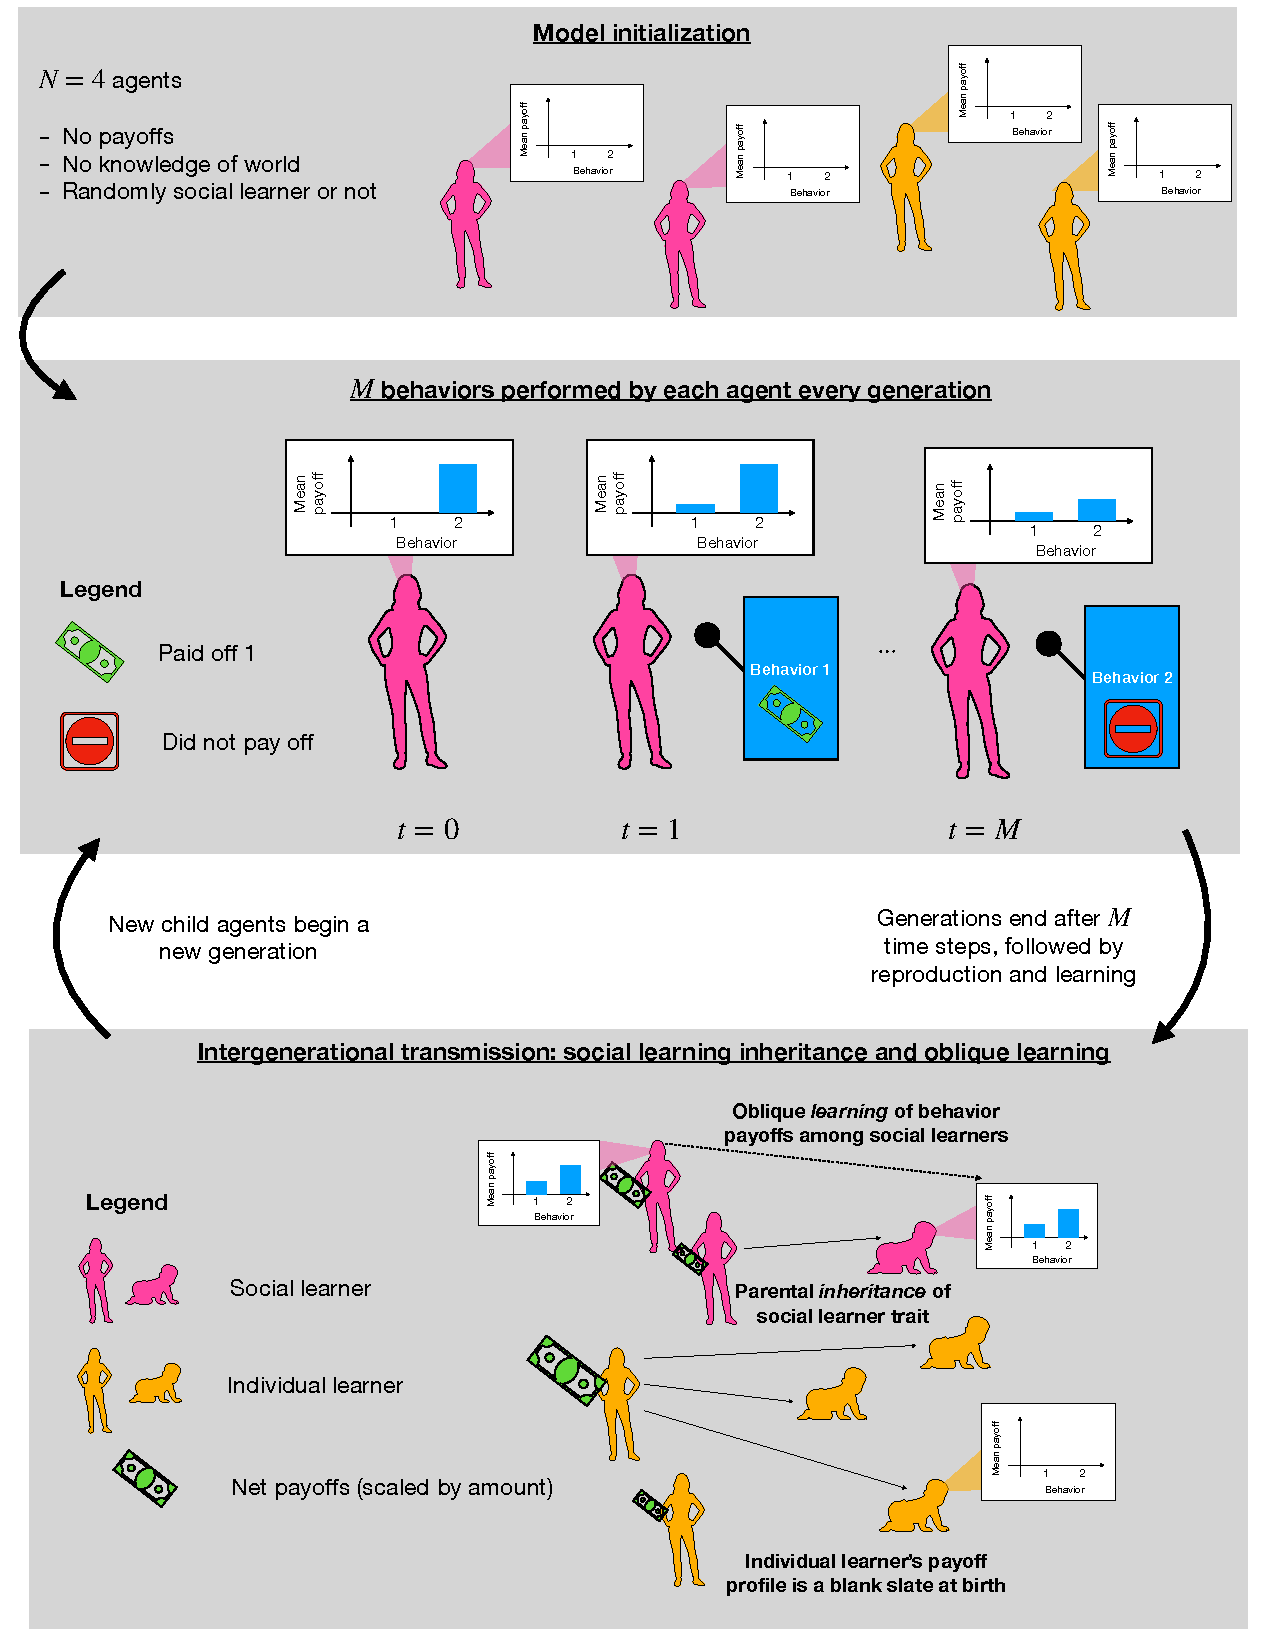
\includegraphics[width=\textwidth]{Figures/IntraInterGenerationalDynamics.pdf}
\end{figure}


\subsection{Computational analyses}
\label{ssec:computationalAnalyses}

% We developed a series of computational
% analyses of the effect of uncertainty on social learning evolution by 
% systematically varying uncertainty parameters and observing how
% frequently model populations evolve to be social learners.  

To analyze the effect of the four principal uncertainty factors, we systematically
varied uncertainty values (Table~\ref{tab:modelParameters}) and observed how frequently social learning evolved across
1000 trial simulations for each combination of parameters tested. %We varied $u \in \{0.0, 0.1, \ldots, 1.0\}$; $\pilow \in \{0.1, 0.45, 0.8\}$; $B \in \{2, 4, 10\}$; and $L \in \{1,2,4,8\}$ for $B=2$ and $L \in \{1,B/2,B,2B\}$ for $B=4,10$.  
We observed three outcome measures, with $\meansl$ as the primary measure: the average value of $s_i$ over all agents and trials. To support our conclusions
about $\meansl$, we also measured $\meanpi / L$, the average net  payoffs at the end of the simulation across agents and trials, normalized by lifespan; 
and $\meanG$, the mean
number of generations to fixation (see Table~\ref{tab:outcomeVariables}). We analyze
outcomes by plotting $\meansl$ on the y-axis and environmental variability on
x-axis, since we
theoretically expect that $\meansl$ will always decrease monotonically from 1 to 0 as $u$
increases. %Note that the hypothesis-testing concept of significance is meaningless here because we could make any small outcome difference ``significant'' by running more simulation trials.  We instead study the patterns of outcome variables over systematically varied uncertainty factor values. 

\begin{table}[h]
    \caption{Outcome Variables. All averages are computed across trials at the end of the last generation.}
    \label{tab:outcomeVariables}
    \centering %\hspace{-3em}
    \begin{tabular}{cp{4.25in}p{0.85in}} \toprule

        Symbol & Description & Values \\ 

        \midrule  

        $\meansl$ & Mean social learning prevalence over agents
                  & $\in [0.0, 1.0]$ \\

        $\meanpi / L$ & Mean payoffs accumulated across agents, normalized by
        lifespan & $\in [0.0, 1.0]$ \\

        $\meanG$ & Mean number of generations to convergence & Unbounded \\
        \bottomrule
    \end{tabular}
\end{table}


\subsubsection{Sensitivity analyses}

We performed sensitivity analyses to ensure that our main analysis is reasonably
robust to a range of auxiliary parameters. These analyses are presented in 
supplemental material. First, we varied the population size, $N$, to confirm that
smaller $N$ would make similar predictions, but with more drift due to finite population size effects. %, but  still generally support our main conclusions. 
Next, we tested model robustness to the number of prospective teachers, $N_T \in \{2, 10, 20\}$, to supplement the main results that used $N_T = 5$. The number of prospective
teachers should not change whether social learning is optimal, but it may induce more drift since the benefit of social learning may
be more difficult to detect with fewer prospective teachers. Finally, we tested
model robustness to varying the
softmax greediness parameter $\beta \in \{1, 100\}$, to supplement the main results
that used $\beta = 10$. We do not
expect agents with different $\beta$ to perform equally well 
individually, so certain $\beta$ values may themselves suppress social learning
by improving or undermining individual learning.  


\subsubsection{Implementation}

Our model was implemented in the Julia programming language~\citep{Bezanson2017} 
using the Agents.jl agent-based modeling library~\citep{Datseris2022} and run
on the Sherlock supercomputing cluster at Stanford University. Model code is
publicly available on GitHub at \url{https://github.com/mt-digital/UncMod},
and output data used to generate the figures presented here are available on OSF.io
\mt{TODO: \url{https://make.OSF.repo}}.


\section{Analysis}

% To understand how different forms of uncertainty interact to affect the evolution of
% social learning, we measured how frequently social learning evolved across
% uncertainty parameters. We analyzed outcomes by plotting the mean observed social
% learning frequency, $\meansl$, with mean taken across all 1000 agents and 1000
% simulation trials for each uncertainty parameter setting at model fixation.
% % This is convenient because we are most certain about how $\meansl$ depends on $u$:
% % we expect $\meansl$ to decrease as $u$ increases since environmental variability
% % is well understood to cause socially-transmitted information to become outdated. 
% % To inspect patterns in $\meansl$ over all uncertainty parameters, 
% We analyze nine plots of how $\meansl$ (y-axis in each plot) changes over 
% environmental variability, $u$ (x-axis),
% in a $3\times3$ plot array (Figure~\ref{fig:mainResults}). 
% % All plots show how $\meansl$ changes (y-axis)
% % with environmental variability, $u$ (x-axis). 
% Selection set size, $B$, increases from left to right in the plot array (columns). 
% Payoff ambiguity increases as the non-optimal payoff, $\pilow$, increases from 
% top to bottom in the array (recall $\pihigh=0.9$ for all analyses).
% Effective lifespan, $L$, is indicated by line and marker colors (inset). 
% Several patterns in social learning prevalence emerged as 
% these uncertainty parameters were varied (Figure~\ref{fig:mainResults}). 


Our main results are illustrated by Figure~\ref{fig:mainResults}, which shows the
proportion of simulation runs that fixated to 100\% social learners as a function of
each of our four uncertainty measures.  First, we found that reliance on social
learning monotonically decreases as temporal environmental variability, $u$,
increases. When the environment is more likely to change between generations,
information learned from the previous generation is less likely to be of value,
decreasing selection for social learning. Past some threshold, social learning is
not favored at all. However, the exact nature of the relationship between social
learning and temporal environmental variability was moderated by the other three uncertainty parameters. 

The number of behavioral options, i.e., larger $B$, favors the evolution of social learning. Increasing the selection set size expands the range of $u$ over which social learning is favored for two reasons. First, when the environment remains constant between generations, the value of social learning increases with more behavioral options, because it effectively increases the number of observations that one can learn from by comparing the payoffs of several models. In other words, relying $only$ on one's asocial trial and error learning is less likely to yield useful information when the search space is large. Second, when the environment changes, bias against the new optimal is weaker with more behavioral options. For example, with only two behavioral choices ($B = 2$), a common assumption in many models, social learning is particularly detrimental when the environment changes since more of the population will have arrived at the optimal behavior in the previous generation and socially learning from them will be biased against the correct choice. These two mechanisms make it particularly profitable to engage in social learning when the selection set size is larger -- for large values of $B$ social learning can even be favored when the environment is more likely to change than not (i.e., $u>0.5$). 

A shorter effective lifespan, $L$, also favors the evolution of social learning in most cases. When effective lifespans are long and there are many opportunities to gather information by learning asocially, the value of social transmission is diminished. Given enough opportunities, all agents will learn the optimal behavior eventually. Thus, under most conditions, longer effective lifespans lead to a narrower range of the parameters $u$ and $B$ under which social learning was favored. It is noteworthy that in many cases, a large increase in the selection regime for social learning could be observed when $L=1$, and by definition no individual learning occurred. The exceptions to this general pattern occur for high levels of payoff ambiguity, $\pilow$ combined with low rates of environmental change, $u$ (left parts of plots on bottom row of Figure~\ref{fig:mainResults}). This reversal is partially explained by higher levels of drift when there is little difference in the payoffs between behaviors, and by the fact that the quality of social information is poorer when payoffs are ambiguous and lifespans are short (more on these effects of payoff ambiguity below).  
% \cm{is this right? I thought we should say something about the exceptions in this paragraph though we describe in more detail below, but not sure I have the right explanation}

Of the four types of uncertainty studied in this paper, payoff ambiguity had the most
complex effect on the evolution of social learning. Recall that we operationalized
payoff ambiguity with $\pilow$, the expected payoff for non-optimal behaviors
(equivalently the probability that those behaviors yielded a payoff of 1). This was
relative to $\pihigh = 0.9$, the expected payoff for the optimal behavior. When
payoff ambiguity was low, non-optimal behaviors rarely paid off, so that exploration
yielded reliable information and selection on learning strategies was  strong. When
payoff ambiguity is very high ($\pilow = 0.8$), two things happen. First, agents are
more likely to err by ascribing high value to non-optimal behaviors, since it is
more difficult for them to discern the difference between optimal and sub optimal
behaviors. Second, and perhaps more importantly, natural selection on strategies
that $do$ reliably select the optimal behavior is relatively weak. This means that
the effect of drift is relatively stronger, weakening selection in favor of social
learning under small values of $u$ and weakening selection against social learning
under high values of $u$ (Figure~\ref{fig:mainResults}, bottom row). 
This effect was especially strong under other types of uncertainty, i.e., larger selection set sizes and especially shorter effective lifespans---particularly when $L=1$ where no individual learning occurred. 

The effect of drift when the benefit of social learning is ambiguous is powerful and complex. We explain how the frequency of social learning evolves in such circumstances in the following section.
%selection on social learning responds to these effects in more detail in the following section. 
%\cm{I rephrased as I didn't think selection was RESPONDING to drift. Original framing sounded weird since in essence we have weak selection which is why drift is relatively high. }



\begin{figure}
  \caption{Social learning prevalence ($y$-axes) monotonically decreases as 
  environmental variability, $u$, increases ($x$-axes) in most uncertainty contexts. 
  Other uncertainty values payoff ambiguity, $\pilow$, (rows), number of behavioral options, $B$, (columns), and effective lifespan, $L$, (keys) shift and flatten the slope from all-social-learner populations to all-asocial-learner
  populations.}
  \label{fig:mainResults}
  \centering
    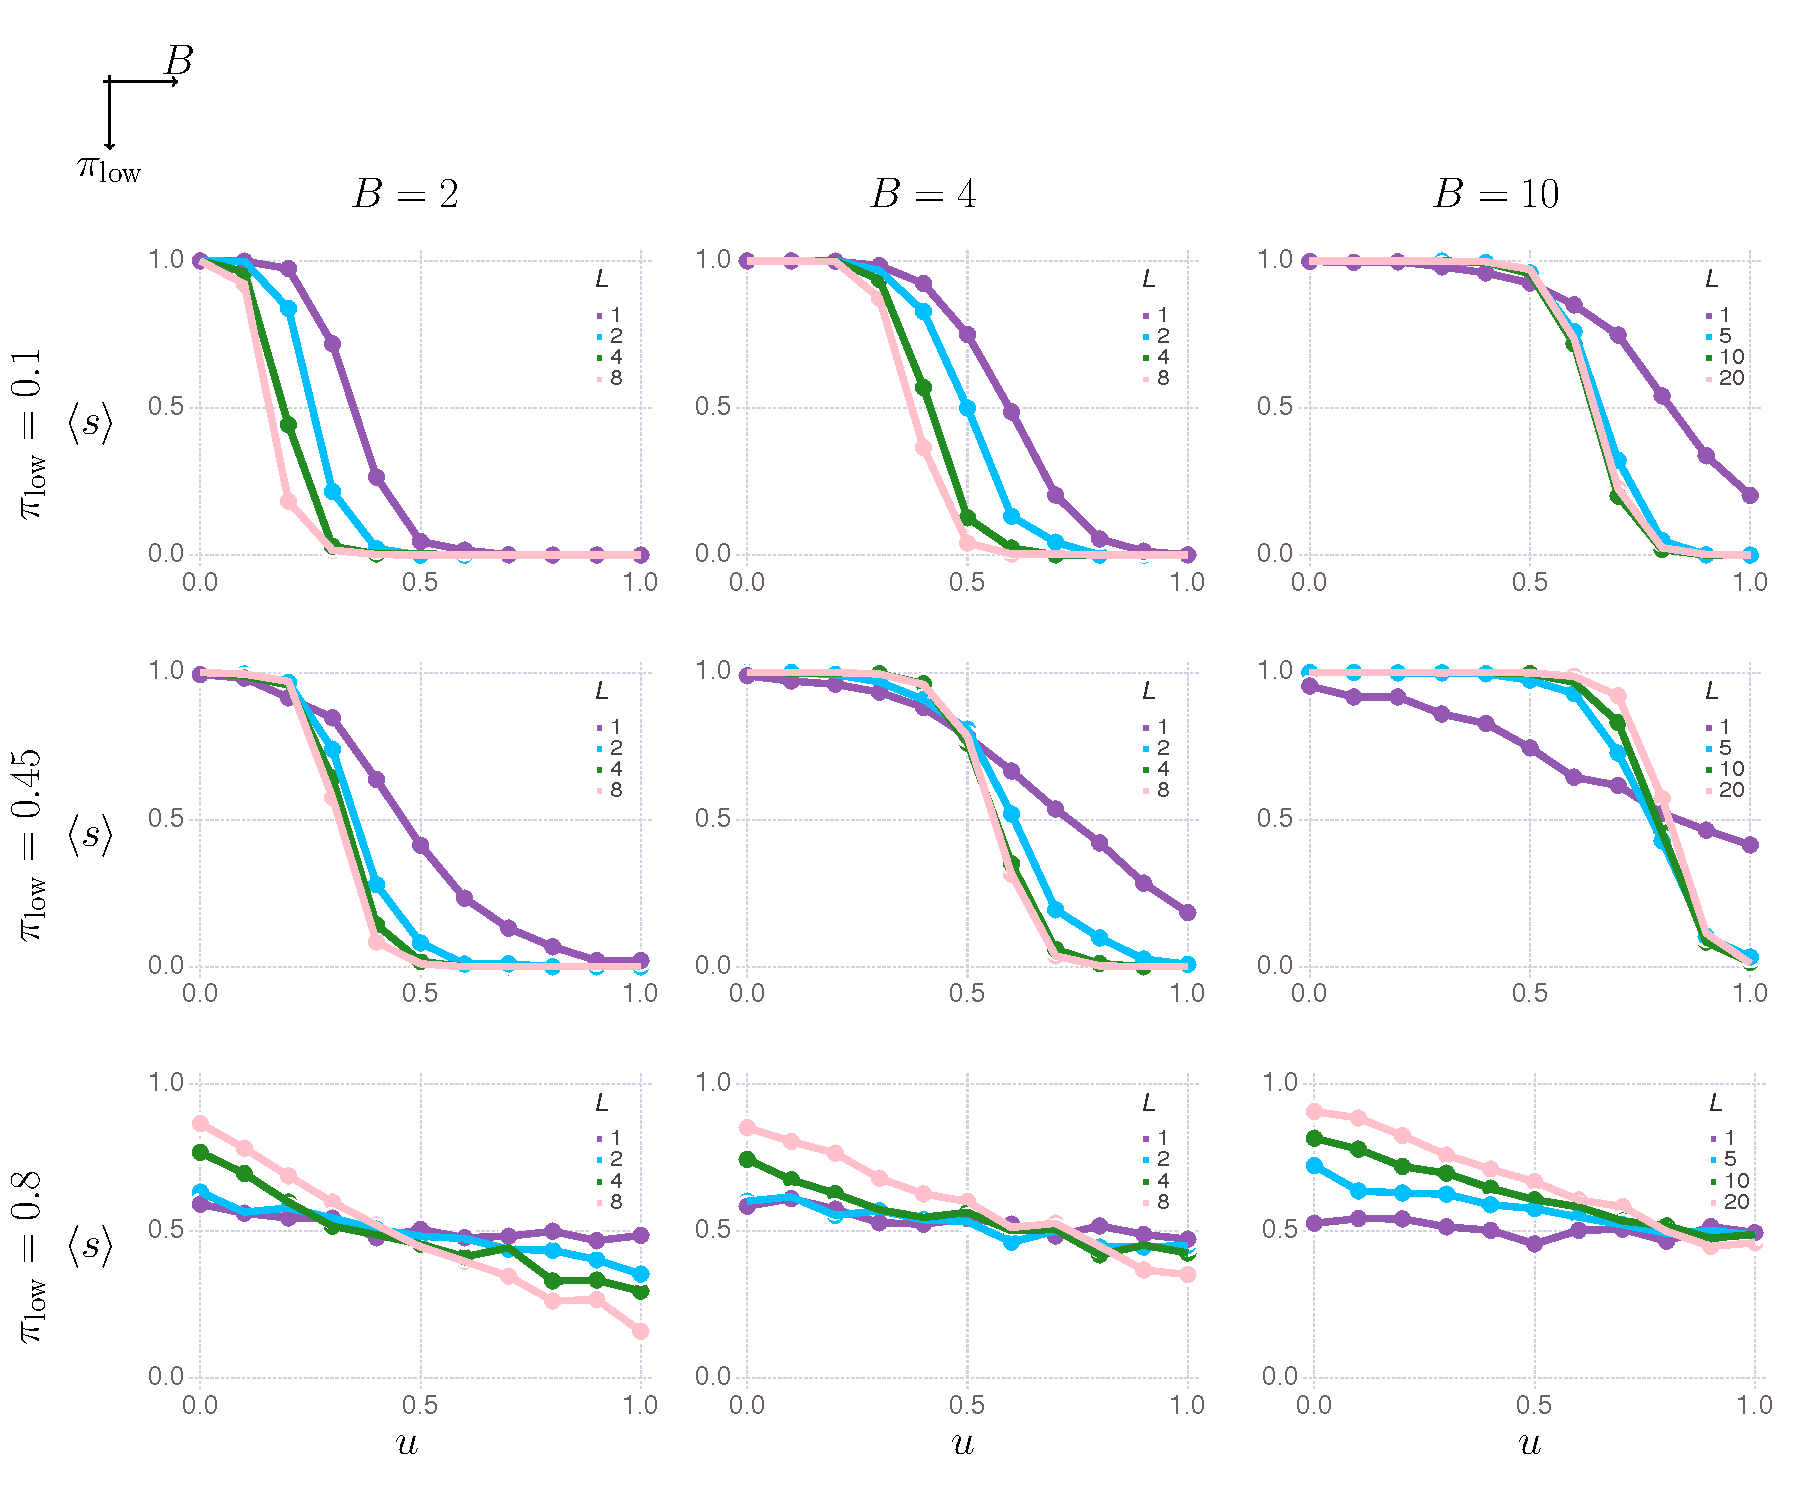
\includegraphics[width=\textwidth]{Figures/mainResultsPlots.pdf}
\end{figure}

\subsection{Evolutionary drift and the relative benefit of social learning}

The effect of drift on the evolution of social learning %evolution and evolutionary drift 
depended on the strength of natural selection, that is, on the extent to which the
social learning trait provided agents with a consistent benefit. Drift infuses
randomness into natural selection. In this model, such randomness is introduced at
various stages including when agents receive payoffs for a given behavior, when they
are reproducing, and when they are being selected as teachers. Drift is maximal, and
in fact the only evolutionary force in our model, when social and asocial learning
are equally beneficial. Even under consistent but weak selection pressure, drift can cause a population to take longer to reach fixation \citep{plutynski2007drift}. We therefore measured drift by the average number of generations to fixation, denoted $\langle G \rangle$, where fixation means that the number of social learners, $\sum_i s_i$, is equal to either zero or $N$. %Indeed, social learning evolution and drift are reflected in the relative benefit of social learning to asocial learning.  

Figure~\ref{fig:steps} shows drift in terms of the average number of generations to fixation, 
$\meanG$, across all uncertainty
parameters. Drift was greatest overall when payoff ambiguity was greatest, i.e., when $\pilow = 0.8$.
When payoffs are highly ambiguous there is relatively little advantage to the
optimal learning strategy, and therefore relatively weak selective pressure.

$\meanG$ peaks at the values of $u$ where social learning becomes suppressed. 
$B$ and $\pilow$ have the
clearest effects on the location of greatest drift over $u$. $L$ has some effect on the location of peak
drift over $u$, but $L$ also has a large effect on the overall amount of drift: $L=1$ tends to have the most
drift with sufficiently low payoff ambiguity ($\pilow < 0.8$). The effect of lifespan on drift is
non-monotonic, since we observe that long lifespans can also result in relatively greater drift
compared to lifespans other than $L=1$ (e.g., in Figure~\ref{fig:steps}, top left and right).
When $L=1$ selection pressure may be relatively weak since agents have no opportunity
for individual learning, and social learning is the only learning channel. 
When $L=8$ ($B=2,4$) or when $L=20$ ($B=10$), individual learning has many 
opportunities for finding the optimal behavior, which means social learning
provides a relatively weaker constraint on net payoffs over agent lifespans.
This also results in weaker selection pressure since there is relatively little
difference between social and asocial constraints when $L$ is large
(Figure~\ref{fig:steps}, top two rows).

We also tracked and analyzed average net payoffs of agent populations across
all uncertainty parameters, and compared the simulated payoffs to 
homogenous all-social learner or all-asocial learner populations. Homogenous payoffs
were calculated by initializing simulation populations to be all social or all asocial learners,
then running the model for 100 generations so payoffs could stabilize; we then averaged 
the net payoffs from the final generation across 1000 trials to calculate the average
homogenous payoffs.

Figure~\ref{fig:payoffs} shows the average net payoffs normalized by lifespan
for our simulations compared with the two reference homogenous populations
initialized either as all social or all asocial learners.
Often the simulated payoffs follow the payoffs from the better-performing
homogenous group, but there are several important deviations to understand.
First, we observed frequency dependence of social learning, where 
agents from our main simulations who evolved to be social learners 
outperform agents in the homogenous social learner populations. This is most
pronounced when $L=1$, across all other uncertainty parameters, and even more
pronounced when $\pilow=0.45$ and $B=10$ (Figure~\ref{fig:payoffs}, middle right).
In these cases, the presence of asocial learners before social learning fixated
enabled social learners in our simulations to outperform all-social learner populations.
Frequency dependence of social learning payoffs even pushed social learning to evolve even
when the expected homogenous social learning payoff was less than the expected homogenous
asocial learning payoff (Figure~\ref{fig:payoffs}, middle center $L=1$).
We also observed cases where long-lived populations ($L=4$ and $L=8$) in simple environments
($B=2$) evolved to be individual learners, even though all-social learner populations
outperformed all-individual learner populations (Figure~\ref{fig:payoffs}, upper left).

We explain these deviations from expected homogenous payoffs 
by inspecting time series of individual model runs where we plot the geometric
moving averages (with time window 3) of the payoffs for the whole population, and
for the series of payoffs broken out by asocial/social learner sub-populations; we
compare these mean payoff series to the expected homogenous social and asocial payoffs, the time series of social learner prevalence, and to the timing of environmental changes within the simulation (Figure~\ref{fig:payoffTimeseries}). 
When lifespan was minimal ($L=1$) and environmental variability
was moderate ($u\approx0.5$), the payoff time series show a period of environmental
stability led populations to fixate to social learning, despite individual learning
being the superior long-term strategy (Figure~\ref{fig:payoffTimeseries}a).
When payoff ambiguity and decision set size was small ($\pilow=0.1$ and $B=2$), 
and lifespan was long ($L=4$ and $L=8$),
asocial learning fixated as a hedge against periods of protracted environmental
instability, which caused social learning to frequently provide
outdated information, even though expected homogenous social payoffs are greater than
homogenous asocial payoffs (Figure~\ref{fig:payoffTimeseries}b,c).

%We measured drift by the average number of generations to fixation, $\meanG$. Recall fixation is defined as the population becoming homogenous, composed of all social or all asocial learners. 
% $\meanG$ peaks around the values of $u$ 
% when $\meansoc \approx \meanasoc$, \cm{wait does it? Fig S2 doesn't seem to show the vertical lines mapping on well} which led $\meansl$ to transition from 1 to 0.
% In some cases, especially when $\pilow=0.8$,
% there is no distinct peak in $\meanG$ across $B$ and $L$ settings, 
% indicating little difference in task difficulty across a range of uncertainty
% parameter settings (Figure~\ref{fig:steps}, bottom row).

% First, we confirmed that social learning evolves when the expected payoffs to social
% learners exceed those of asocial learners, which we write $\meansoc > \meanasoc$.
% In the case of $L=1$ we can calculate $\meanasoc$ directly: it is just the expected
% payoff across all behaviors. For all other cases, we calculate expected social and asocial payoffs by respectively setting
% $\sum_i s_i = N$ or $\sum_i s_i = 0$ at model initialization. These populations remain homogeneous since we do not allow for mutation. From these runs we calculate the payoffs to a population of either all social learners or all asocial learners after x generations \cm{you waited for them to stabilize or something right? only relevant for social learner population, but needs some more explanation}.  Figure~\ref{fig:payoffs} shows these expected payoffs, normalized by effective lifespan $L$), as well as the observed average payoffs in our simulations. \ps{Is this right? I'm having trouble understanding what the solid lines in Figs 3 and 5 are. I'm also debating the wisdom of separating these figures. Maybe we put the 3x3 back in for Fig 3?}
% In general, we observed that social learning evolved in our simulations when the expected payoffs exceeded expected individual-learner
% payoffs (Figure~\ref{fig:payoffs}). This mapping of expectations to model results is reflected in Figure~\ref{fig:mainResults} given the vertical lines map onto the transitions from social to asocial learning in the curves. \cm{wait i wrote this and then noticed that I was looking at the wrong vertical lines (the <G> ones) now I'm confused.}

\begin{figure}
  \caption{Average number of generations ($\meanG$, y-axes) to fixation. 
    Note the y-axis ticks vary between plots, indicating different overall 
    time to fixation for different $(\pilow, B)$ pairs.} 
  \label{fig:steps}
\centering
    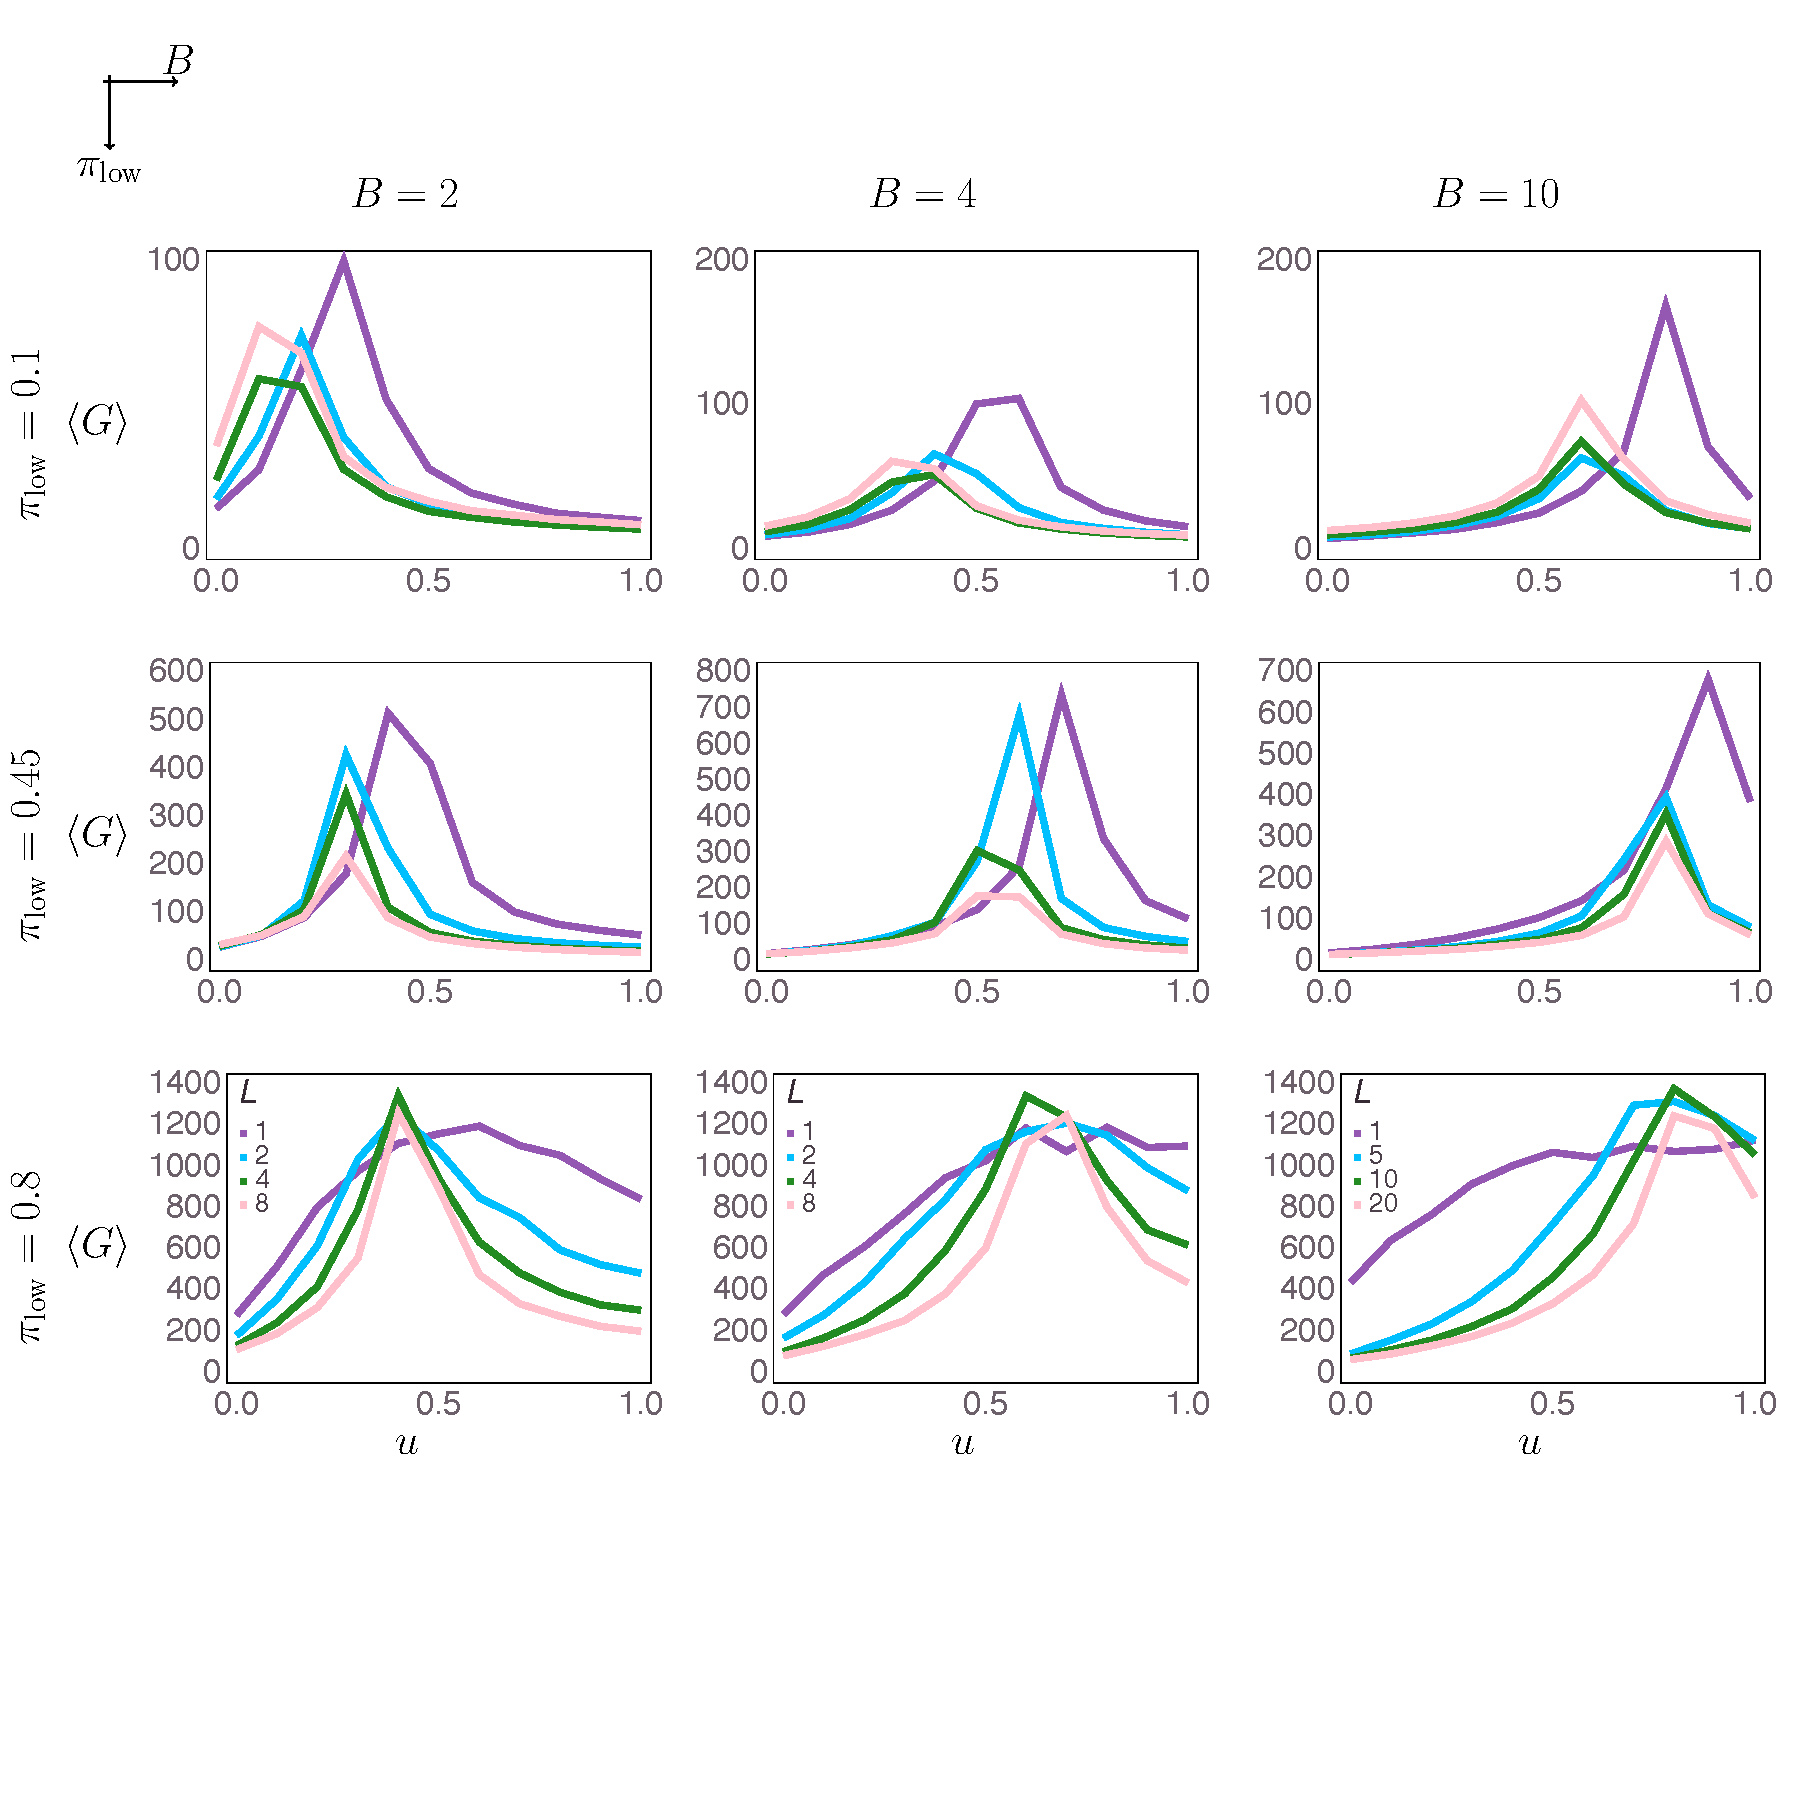
\includegraphics[width=\textwidth]{Figures/stepResultsPlots.pdf}
\end{figure}

\clearpage
\begin{figure}
  \caption{Comparison of observed average payoffs in simulations with average payoffs
    obtained by populations homogenously initialized to be all social or all asocial learners.
    Often the simulated payoffs follow the payoffs from the better-performing
    homogenous group, with some exceptions discussed in the main text.
}
  \label{fig:payoffs}
  \centering
    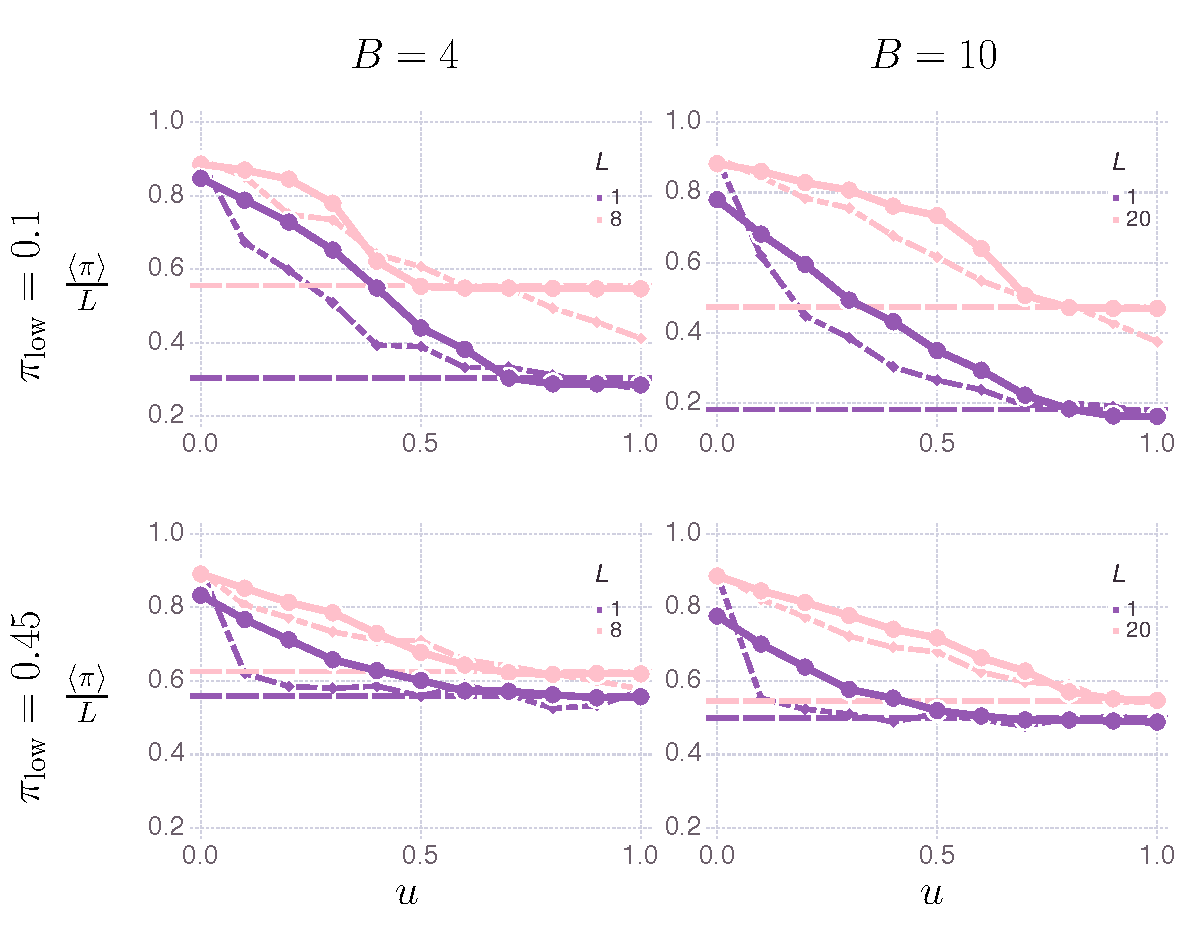
\includegraphics[width=\textwidth]{Figures/meanNetPayoffs.pdf}
\end{figure}


\begin{figure}
    \caption{Example time series of geometric moving average (GMA) with window of 3
      of payoffs from three select uncertainty settings (see main text), broken out by 
    social learners, asocial learners, and whole population, compared with the
    expected homogenous social and asocial population payoffs. 
    Social learner prevalence is also plotted. Vertical lines indicate
  environmental change.}
    \label{fig:payoffTimeseries}
  \centering    

\vspace{1em}
\hspace{-2em}
    \begin{subfigure}[]{0.75\textwidth}
      \centering
    \caption{$\pilow=0.1$, $B=4$, $L=1$, $u=0.5$}
      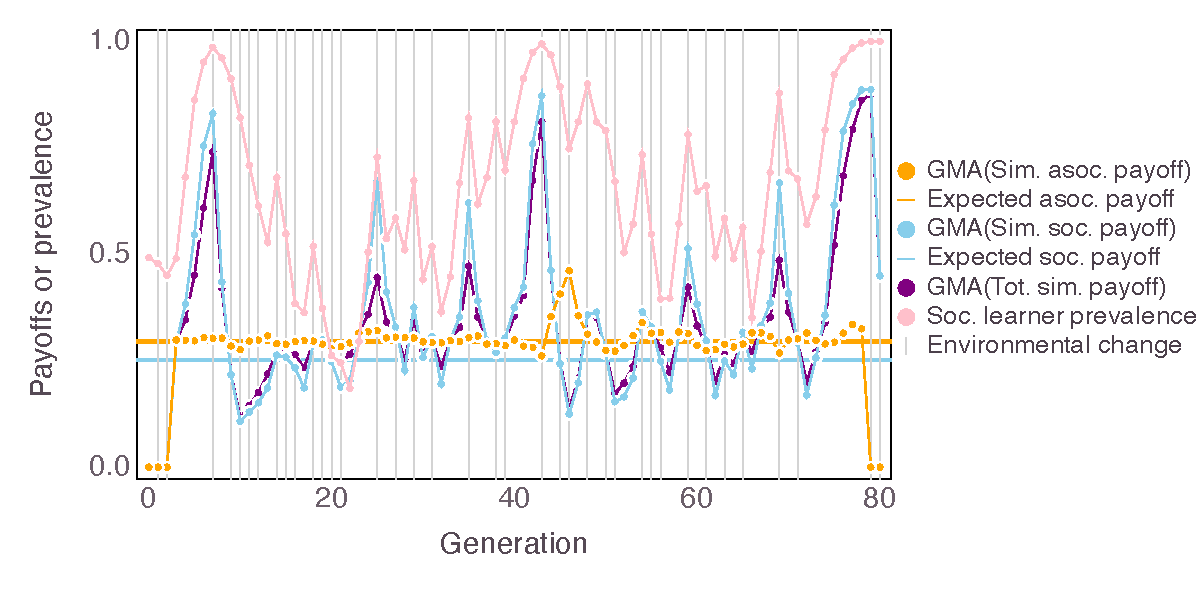
\includegraphics[width=0.95\textwidth]{Figures/geopayoff_series/geopayseries_u=0.5-lowpayoff=0.1-nbehaviors=4-L=1.pdf}
    \end{subfigure} \\
    
\hspace{-2em}
  \begin{subfigure}[]{0.75\textwidth}
      \centering
      \caption{$\pilow=0.1$, $B=2$, $L=4$, $u=0.2$}
      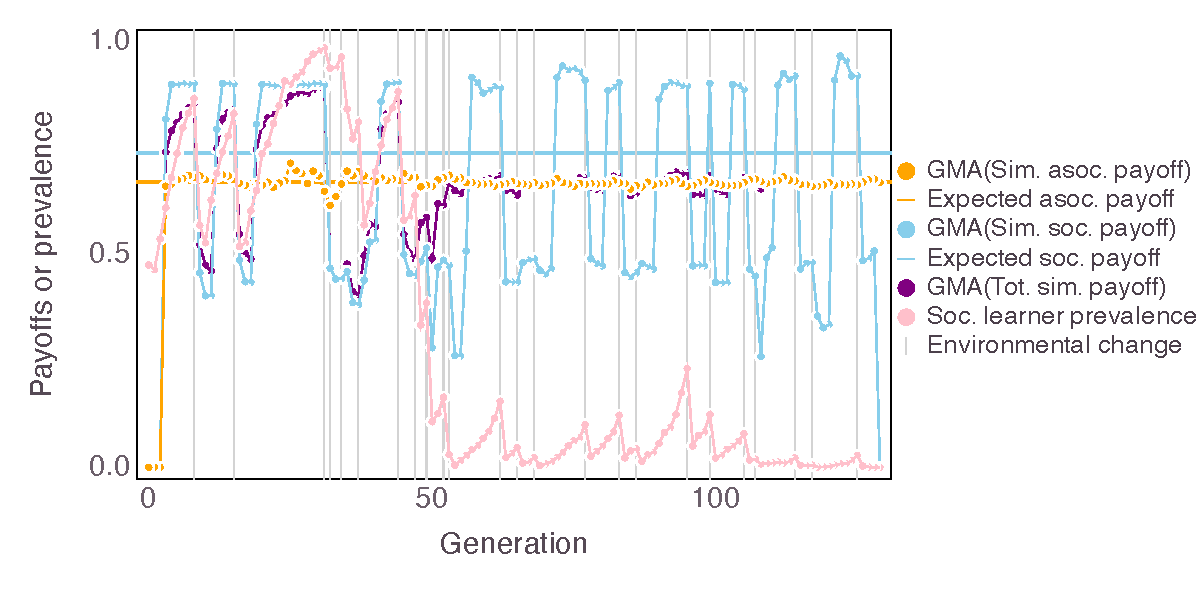
\includegraphics[width=0.95\textwidth]{Figures/geopayoff_series/geopayseries_u=0.2-lowpayoff=0.1-nbehaviors=2-L=4.pdf}
    \end{subfigure} \\

\hspace{-2em}
    \begin{subfigure}[]{0.75\textwidth}
      \centering
      \caption{$\pilow=0.1$, $B=2$, $L=8$, $u=0.2$}
      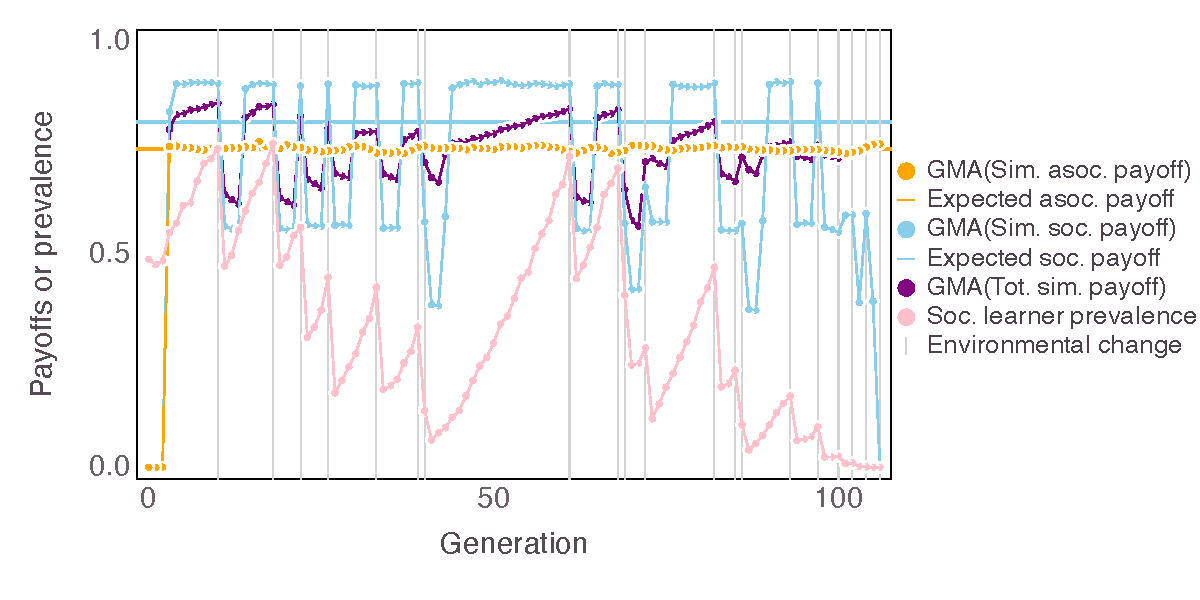
\includegraphics[width=0.95\textwidth]{Figures/geopayoff_series/geopayseries_u=0.2-lowpayoff=0.1-nbehaviors=2-L=8.pdf}
    \end{subfigure}


    % \\
    % \begin{subfigure}[]{0.6\textwidth}
    %   \centering
    %   \caption{$\pilow=0.1$, $B=10$, $L=20$, $u=0.5$}
    %   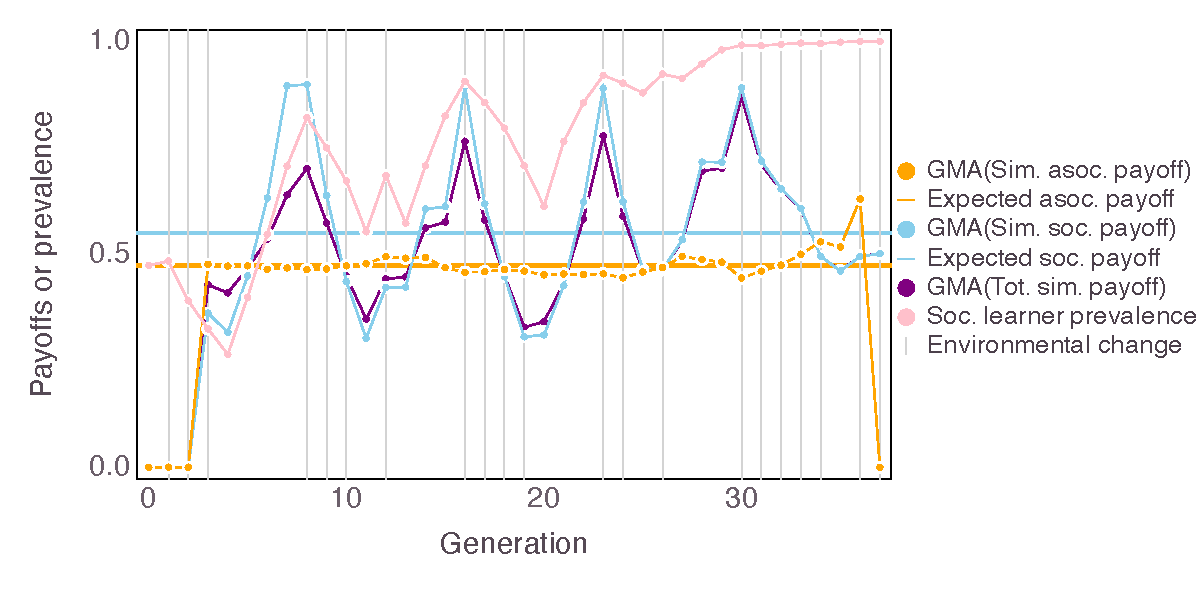
\includegraphics[width=0.95\textwidth]{Figures/geopayoff_series/geopayseries_u=0.5-lowpayoff=0.1-nbehaviors=10-L=20.pdf}
    % \end{subfigure}
\end{figure}




\section{Discussion}

 Despite the common claim that copying others makes sense when one is uncertain, we find that different forms of uncertainty can either promote, or impede, the evolution of social learning. By disambiguating various formalizations of uncertainty in a single computational model, we have developed a more nuanced theoretical understanding of how uncertainty affects the evolution of social learning.
%We reviewed and distilled several empirical and theoretical models in the literature along four uncertainty dimensions: temporal environmental uncertainty, selection set size, ambiguous payoffs, and effective lifespan.  
We reproduced the well-known results that the uncertainty derived from a temporally variable environment can limit the evolution of social learning if environmental change is simply too rapid for intergenerational transmission to be of value. Importantly, we also showed that this relationship is affected by other sources of uncertainty. 
%Our model reproduced classic predictions that social learning can yield higher payoffs than individual learning when uncertainty is sufficiently limited. 
We found that larger sets of behavioral options, shorter effective lifespans, and increased payoff ambiguity could all favor the evolution of social learning. However, these effects were not always straightforward. 
Increased payoff ambiguity and decreased effective lifespan afforded a greater role for drift, which is essentially
evolutionary uncertainty in a finite-size population. Not surprisingly, when the consequence of one's choice does not affect payoffs much, selection either for or against social learning is substantially weaker. More interestingly, selection is also weaker when the ability to learn asocially is fraught with uncertainty. Our model demonstrated that social learning can act as a scaffold for individual learning---they are not opposite strategies. We endowed agents with a biologically-plausible individual learning mechanism, softmax search. This enabled agents to recover from the potential cost of receiving outdated information. This in turn enabled the evolution of social learning even when social information was likely to be outdated. 

% \cm{this seems to say the opposite of the topic sentence. In topic sentence social learning-> asocial, but the mechanism descibed later is asocial learning -> social. Both seem possible, though the latter is easier for me to understand.}

Our modeling results suggest, on the one hand, that society might be better to
ignore social information from previous generations since our natural world is
rapidly changing~\citep{IPCC2022}; on the other hand, humans have increasingly more
behavioral options (selection set size) with high levels of uncertainty about which behaviors are most beneficial (payoff ambiguity), and in this case our model predicts a greater prevalence of social learning.
In general, detailed theoretical models like this are likely to be critical for understanding how humans might adapt to an uncertain and rapidly changing world.
Such understanding could suggest plausibly beneficial interventions to mitigate existential threats~\citep{Moya2020,Jones2021}, especially in
the most vulnerable communities~\citep{McNamara2020}, and to capitalize on new behavioral opportunities such as transitioning to clean energy use and
production~\citep{NatureEnergyEditorialPromisesPremises2018,Brisbois2022}. However, to better identify
potential pathways to effective adaptation it may be necessary to adjust some of our modeling assumptions to
include both the cumulative nature of cultural evolution and group structure of interpersonal exchange, both
of which have been shown to affect the sustainability of novel adaptations~\citep{Derex2020,Centola2018,Smaldino2021a}.
\cm{should we draw out some implications? I find this difficult, but e.g. stressing environmental change may discourage learning from older gen? having more tech options available for dealing with climate change may encourage social learning? Frankly so many of these problems seem to come back to encouraging people to socially learn from the RIGHT people, not just socially or asocially learning.} \mt{I gave this a try, with some restructuring to put the note about social learning as a scaffold for individual learning in the above paragraph.}

Our model necessarily made simplifying assumptions. These were chosen judiciously to address the main
question of how uncertainty affects the evolution of social learning. Two critical assumptions we made have
important consequences for comparing our results with previous findings in the literature. First, we assume
all agents engage in individual learning. This means that individual learning is effectively free, though
potentially inaccurate. Although producing new knowledge may be costly, many other adaptive problems take
the form of essentially cost free individual learning. For example, one cannot help but experience the association between; clouds and rain, thirst and drinking water, or smiling and
being avoided. This model thus avoids scrounger/producer dynamics common in other models
~\citep{BoydRicherson1985,Rogers1988} and therefore does not produce any mixed equilibria of social and
asocial learners.  Second, we only allow for intergenerational social learning and environmental change.
Within generations agents can only learn asocially, meaning they cannot learn from their peers. This
assumption allows us to replicate the classic finding that if the environmental change too quickly, socially
learned information will be useless. Alternative formalizations for the timing of social learning and
environmental change would break this relationship~\citep{Turner2022}. 

We could have made alternative, empirically-valid, choices for a range of other structural features, the future exploration of which will be important to the development of a more nuanced theory of social learning.  % that may not always hold in more specific situations, though they are empirically justified to be general across taxa. 
For example, we only considered success-biased
learning, although people may use conformity or other context biases to socially
learn~\citep{BoydRicherson1985,Muthukrishna2016a,Smaldino2018b}.  This modelling
choice maximizes the potential benefit to social learners, which suggests that
other mechanisms, like conformity, may lead to more drift overall. We also assumed that the number of behaviors and
their payoffs were constant within a given simulation, but this fails to account for evolutionary feedback which creates new behavioral opportunities as time progresses, e.g.\ via niche construction~\citep{Smaldino2012a,Heras-Escribano2020} or cumulative cultural evolution
%supported by dynamic network structure
~\citep{Smolla2019,Derex2020}.  Group structure
and processes such as homophily and other group-level biases could inhibit the
evolution of social learning since successful out-group teachers could be cut off from
in-group learners~\citep{Golub2012}. We assumed agents choose behaviors via softmax
search, but even though this algorithm is more sophisticated than most used in social learning models, it is algorithm compared to real human learning mechanisms ~\citep{Schulz2020a,Wu2022}. Instantiating even more powerful asocial learning could further
support the evolution of social learning. These considerations reveal new opportunities to enhance theoretical nuance by adjusting or extending the present model for other contexts. 


%\subsection{Conclusion}

%We found that the 
The evolution of social learning is a complex phenomenon, dependent on many interrelated factors. Although social learning is widely studied, few studies have previously examined how various environmental variables contributing to uncertainty interact. 
By carefully identifying and operationalizing common forms of  uncertainty in social learning models, we developed a more systematic
understanding of which uncertainty factors interact to determine whether social
learning evolves. By explicitly modeling a key individual-level learning mechanism
shared across taxa, namely the ability to adjust behavior to uncertainty and new
information, we saw that social learning could evolve even if social learning
often provides outdated information. 

Social learning is a critical component of problem solving among social creatures.
Our work identified and systematized some important forms of uncertainty and catalogued their effects on 
the evolution of social learning. Our work, then, both advances the theory of social
learning and could eventually be of practical use in designing sustainable
adaptations to an uncertain future.
% This work most directly informs our current understanding of the evolution of social learning, but also has broader significance for understanding problem solving under uncertainty. 
\ps{What is this significance? Can't just leave that dangling. I also cut the bit about what comes next. No need for spoilers.} \mt{Gave this a try, but I think Jamie should have a crack at this.}
%Our model and its software implementation were designed to be modular and extensible.  Indeed, we plan to extend this model to further develop a more detailed theoretical understanding of the evolution of social learning; we hope others will, too.


\bibliographystyle{apalike} %cite}
% \bibliography{/Users/mt/workspace/Writing/library.bib}
\bibliography{this.bib}


%%%%%%%%%% Merge with supplemental materials %%%%%%%%%%
\pagebreak
\begin{center}
  \textbf{\Large \textsf{Supplement}}
\end{center}
%%%%%%%%%% Merge with supplemental materials %%%%%%%%%%
%%%%%%%%%% Prefix a "S" to all equations, figures, tables and reset the counter %%%%%%%%%%
\setcounter{equation}{1}
\setcounter{figure}{0}
\setcounter{section}{0}
\setcounter{table}{0}
\setcounter{page}{1}
\makeatletter
\renewcommand{\theequation}{S\arabic{equation}}
\renewcommand{\thefigure}{S\arabic{figure}}
\renewcommand{\thetable}{S\arabic{table}}
\renewcommand{\thesection}{S\arabic{section}}
\renewcommand{\thepage}{S\arabic{page}}
% \renewcommand{\bibnumfmt}[1]{[S#1]}
% \renewcommand{\citenumfont}[1]{S#1}
%%%%%%%%%% Prefix a "S" to all equations, figures, tables and reset the counter %%%%%%%%%%




% \section{Additional main figure: Full net payoff comparison for all nine uncertainty conditions} 
% \ps{This should be part of the supplement. Also, all supplementary figures and tables should be preceded by ``S".}
% In the main text we showed a $2\times2$ array of plots comparing the observed
% mean net payoffs obtained by agents in our simulations, and in two auxiliary
% sets of simulations that set all agents to either have the social learning
% trait or not, which remained the case for the entire simulation since there
% are no mutations in this model (Figure~\ref{fig:payoffs}). Here we show the full $3\times3$ array of
% all $(\pilow, B)$ combinations shown for the main results. We see that
% populations of all social learners especially underperform initially mixed
% populations that evolve to be social learners 
% (Figure~\ref{fig:fullMeanPrevNetPayoffs}, bottom row). This highlights the
% importance of diversity for behavioral optimization, even if it is transient.


% \newpage



In this Supplement we support our model conclusions by showing that our model
outcomes are stable over various settings of the three free auxiliary model
parameters: the number of agents ($N$), the number of
prospective teachers which social learner children compare
($N_T$), and the softmax behavior selection greediness parameter ($\beta$).
The main source of minor deviations from the main results was greater drift
due to (1) finite population size effects, with greater drift for smaller $N$;
(2) lower quality of socially-learned information when agents can access fewer
prospective teachers; and (3) lower quality social information when $\beta$
was small since teacher agents would have explored non-optimal behaviors more
frequently, so their observed payoffs would have less probability weight in
the optimal payoffs on average. We give details below of model convergence, and
outcomes as we varied the three auxiliary parameters $N$, $N_T$, and $\beta$.

% \section{Expected payoffs}

\clearpage



\newpage

\section{Population size sensitivty analysis}

Drift was greater for smaller populations sizes, especially when $\pilow=0.8$, but 
the main patterns are robust with greater finite population size effects, specifically
with $N=50$ and $N=200$ (recall $N=1000$ tested in main analysis). 
Drift is also more pronounced for smaller $N$
for shorter lifespans, especially $L=1$. When $L=1$ and $N=50$ , the S-shaped
curve of $\meansl$ over $u$ becomes more linear with increasing $B$, 
with $\meansl$ values pulled towards maximal drift, $\meansl \to 0.5$ (Figure~\ref{fig:populationSensitivity}a,
purple curves). With
$N=50$, all $\meansl$ over $u$ curves are flattened with less sharp transitions
from $\meansl = 1$ for lesser $u$ to $\meansl = 0$ for greater $u$. Despite
these finite-population effects, we still see the inhibition of social learning
as $u$ increases, more social learning across $u$ for larger $B$, and the
same complex drift effects for combinations of $\pilow$ and $L$ that interact
with $u$ and $B$ settings.

\clearpage

\begin{figure}
  \centering
  % \addtocounter{figure}{-1}
  \caption{
	Sensitivity analysis of the main results for two population
	sizes, $N=50,200$. Recall $N=1000$ was used to generate main 
	text results.
  }
  \label{fig:populationSensitivity}
  \begin{subfigure}{\textwidth}
	\caption{$N=50$}
	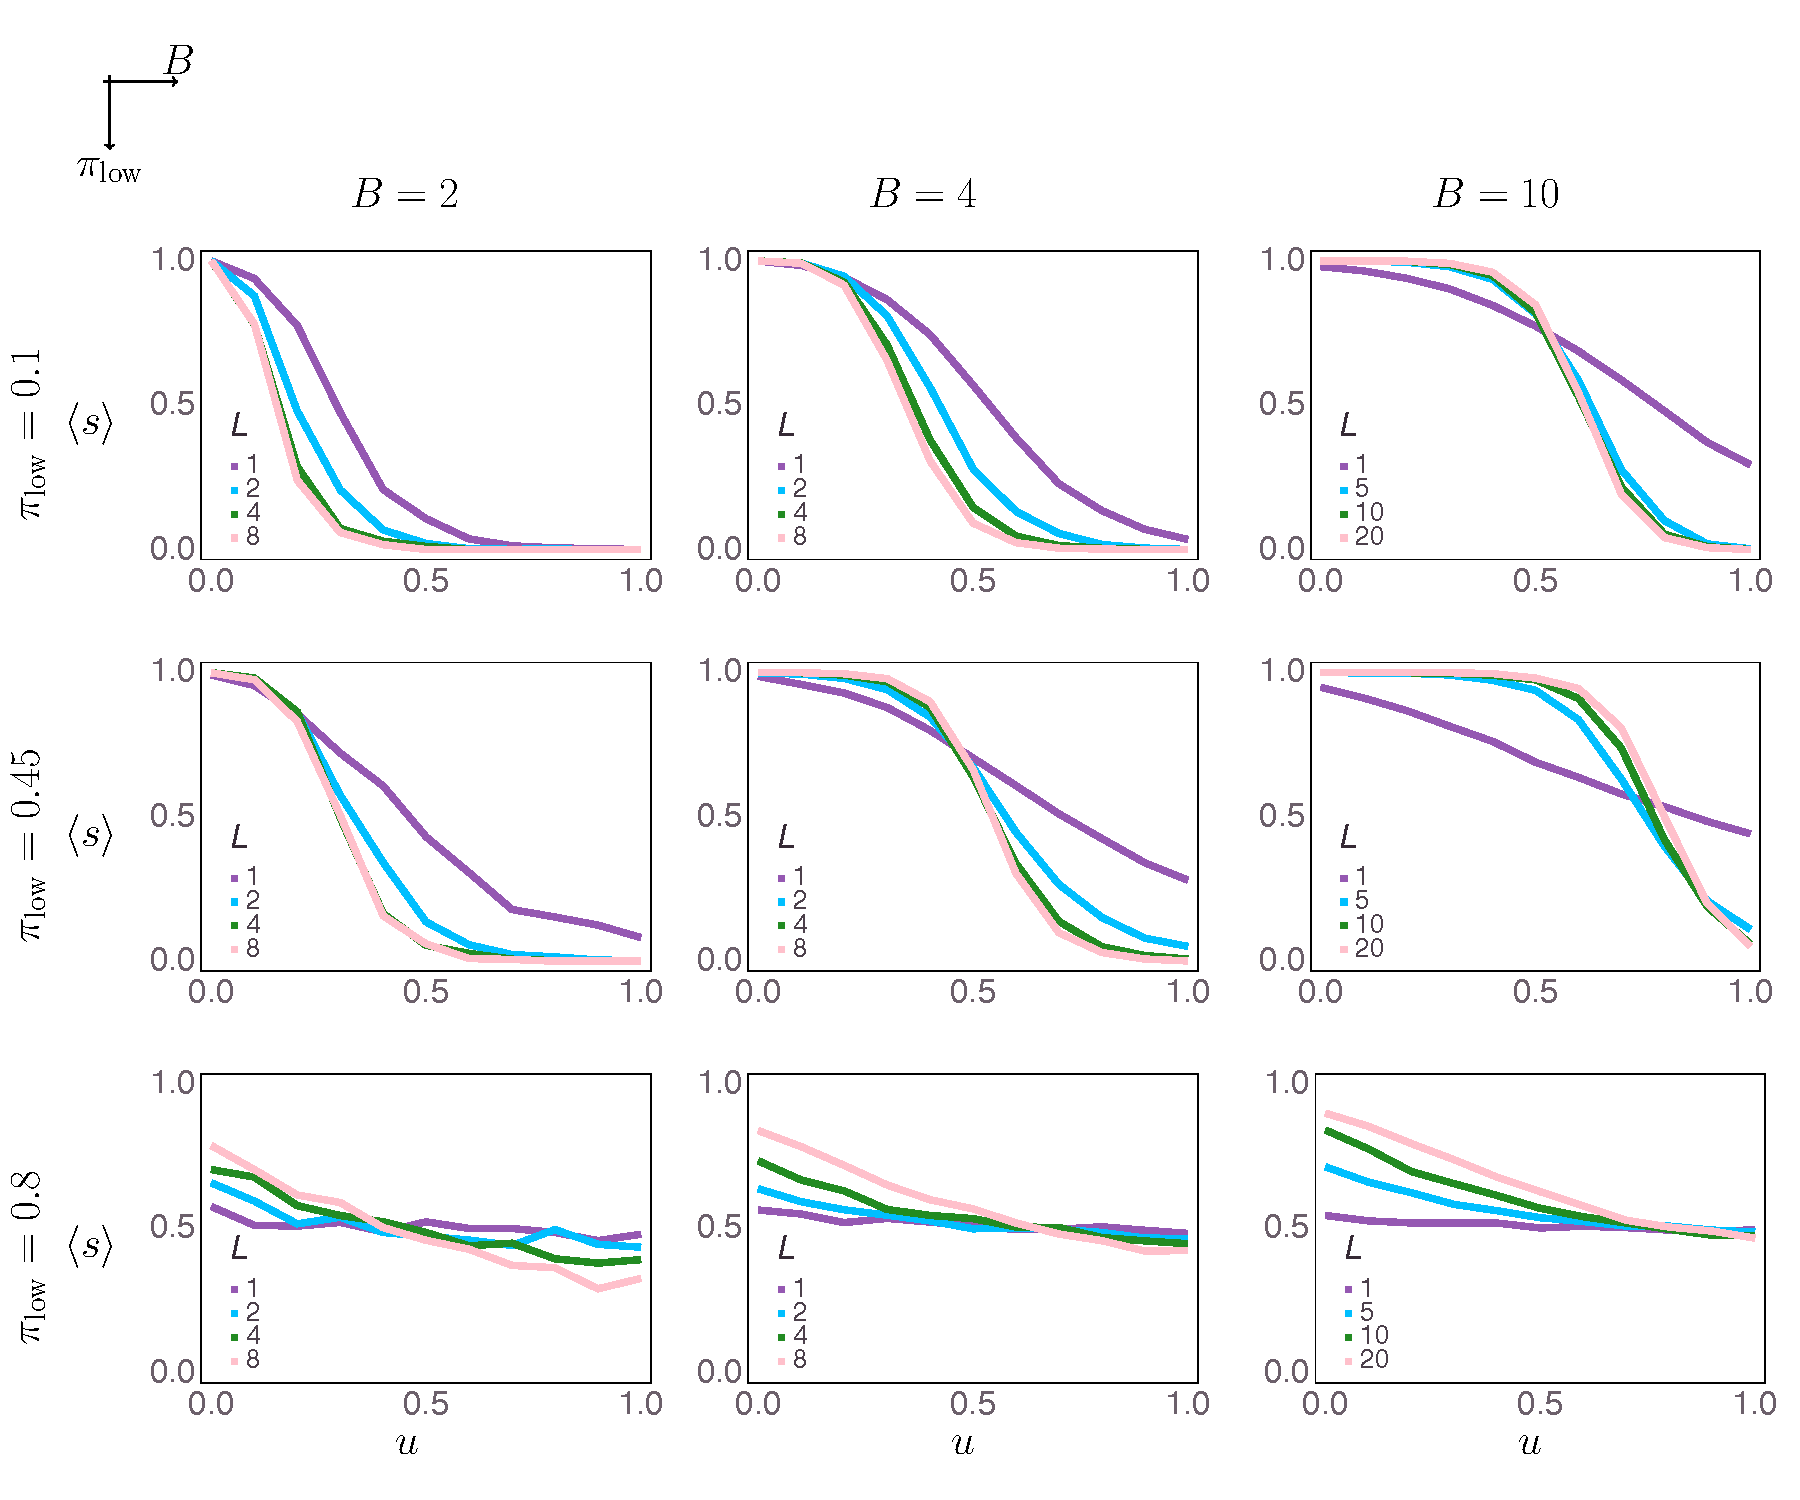
\includegraphics[width=\textwidth]{Figures/supplement/numagents=50/mainResultsPlots.pdf}
  \end{subfigure}
\end{figure}

\begin{figure}
  \ContinuedFloat
	\begin{subfigure}{\textwidth}
	  \caption{$N=200$}
	  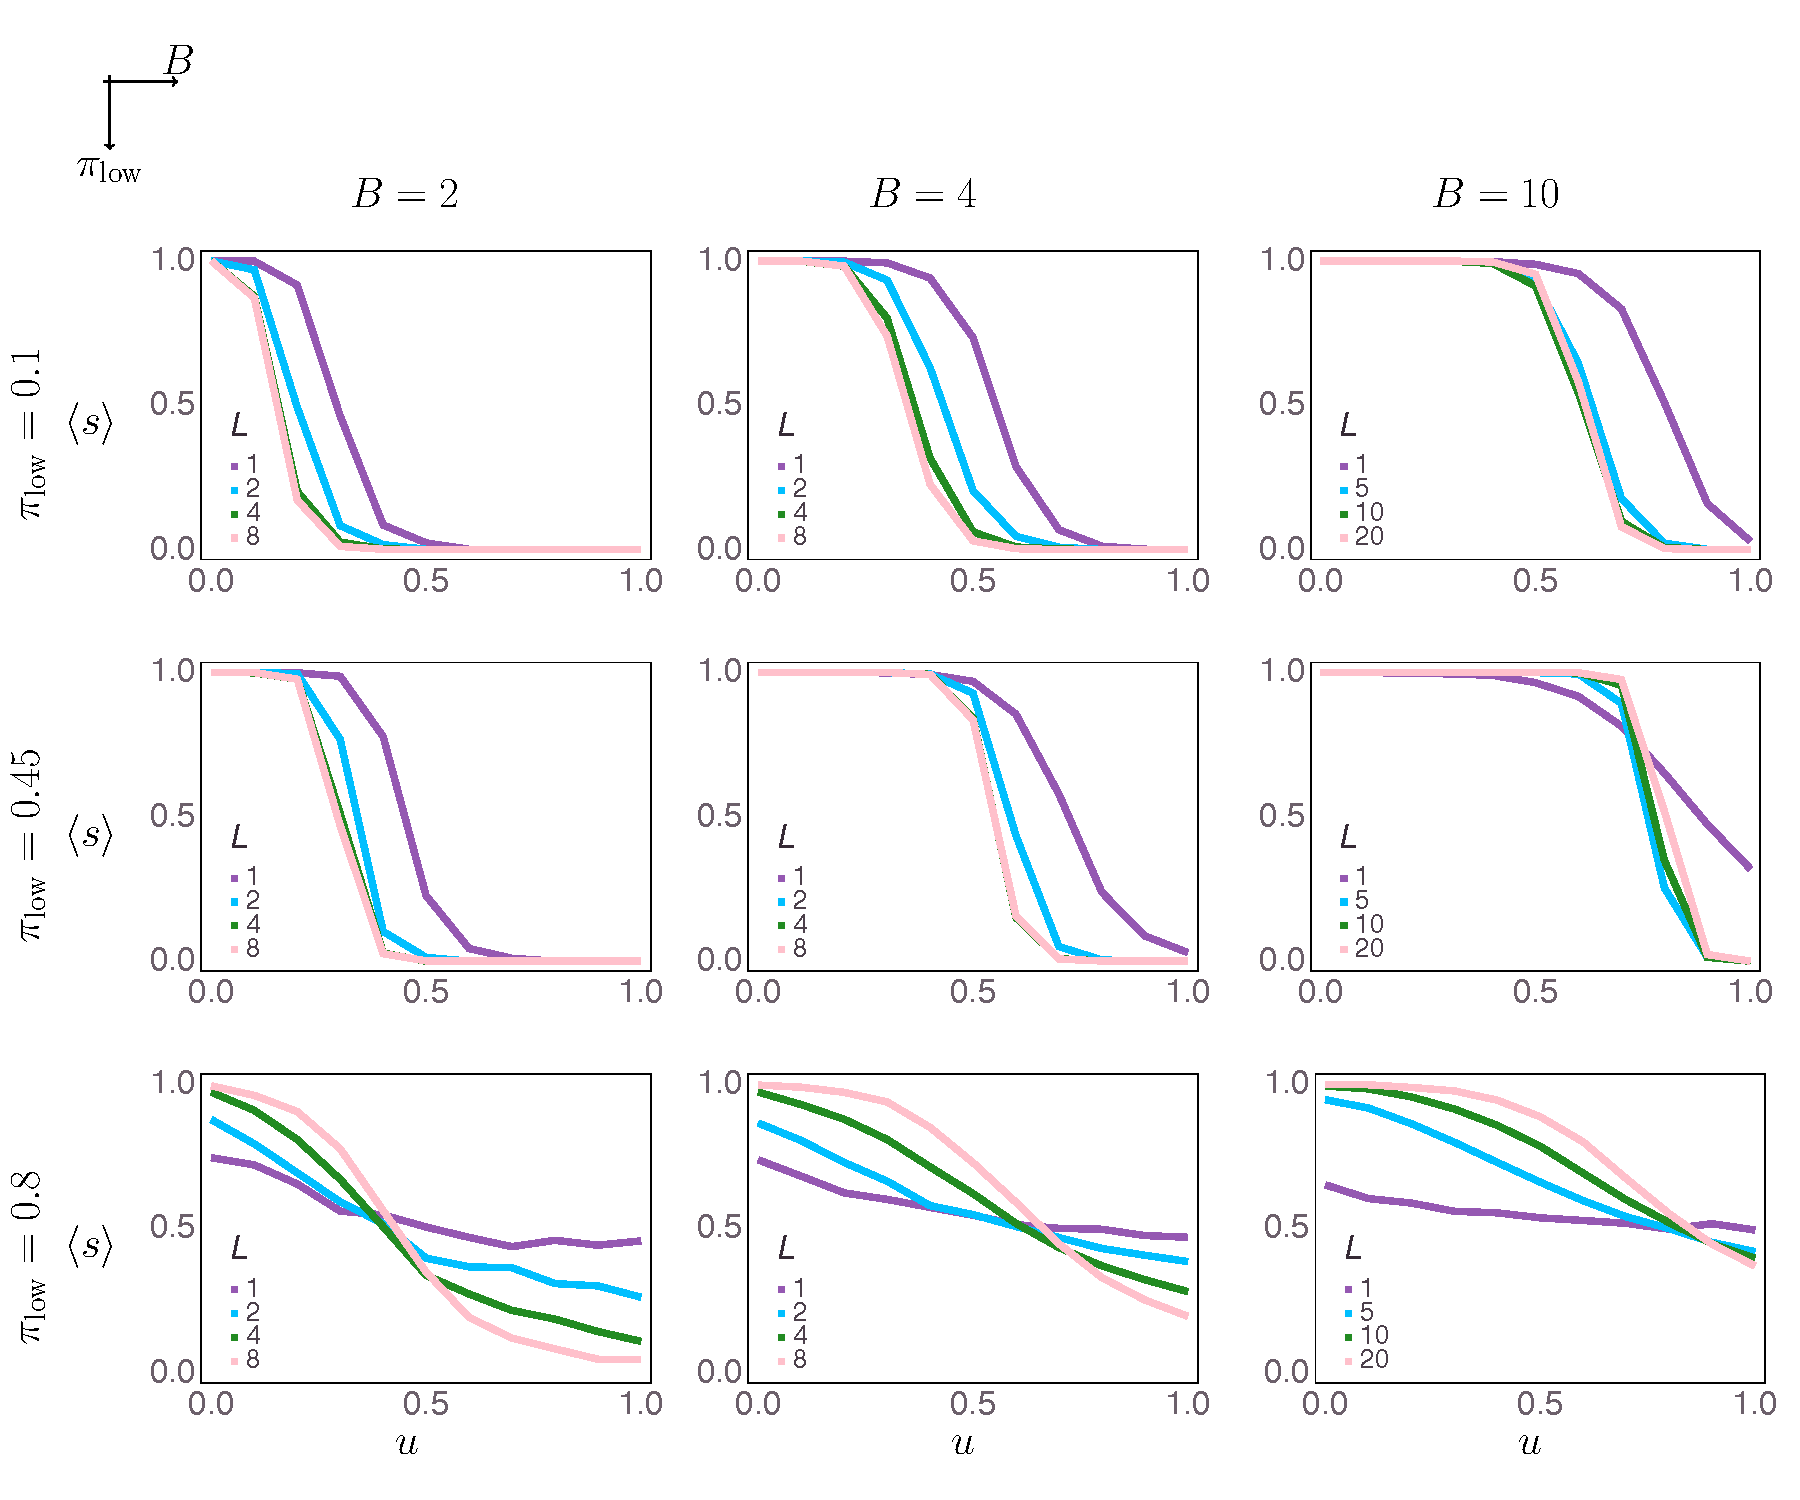
\includegraphics[width=\textwidth]{Figures/supplement/numagents=200/mainResultsPlots.pdf}
	\end{subfigure}
\end{figure}


\clearpage

\section{Number of prospective teachers sensitivty analysis}

We found that the number of prospectve teachers had little effect on $\meansl$
over $u$. There was slightly more drift when $N_T = 2$ compared to our 
main text analysis, slightly less drift than our main analysis when $N_T = 20$; 
we also tested $N_T=10$, which showed no obvious difference from our main results
with $N_T = 5$. When $N_T = 2$, increased drift is most pronounced in the
$\meansl$ curves when $\pilow=0.8$ (Figure~\ref{fig:nteachersSensitivity}a, 
bottom row). The transition from $\meansl = 1$ to $\meansl = 0$ is less sharp
across $L$ values, with social learning evolution being suppressed beginning
at smaller values of $u$. By contrast, when $N_T = 20$, transitions from 
$\meansl = 1$ to $\meansl = 0$ are sharper across $L$ when $\pilow = 0.8$
(Figure~\ref{fig:nteachersSensitivity}c, bottom row). Otherwise, the main 
results were reproduced across all tested values $N_T=2,5,10,20$.

\clearpage


\vspace{-3em}
\begin{figure}
  \centering
  % \addtocounter{figure}{-1}
  \caption{Number of prospective teachers sensitivity analysis for $N_T=2,20$. Recall
  $N_T=5$ was used to generate main text results.}
  \label{fig:nteachersSensitivity}
  \vspace{2em}
  \begin{subfigure}{\textwidth}
	\caption{$N_T = 2$}
	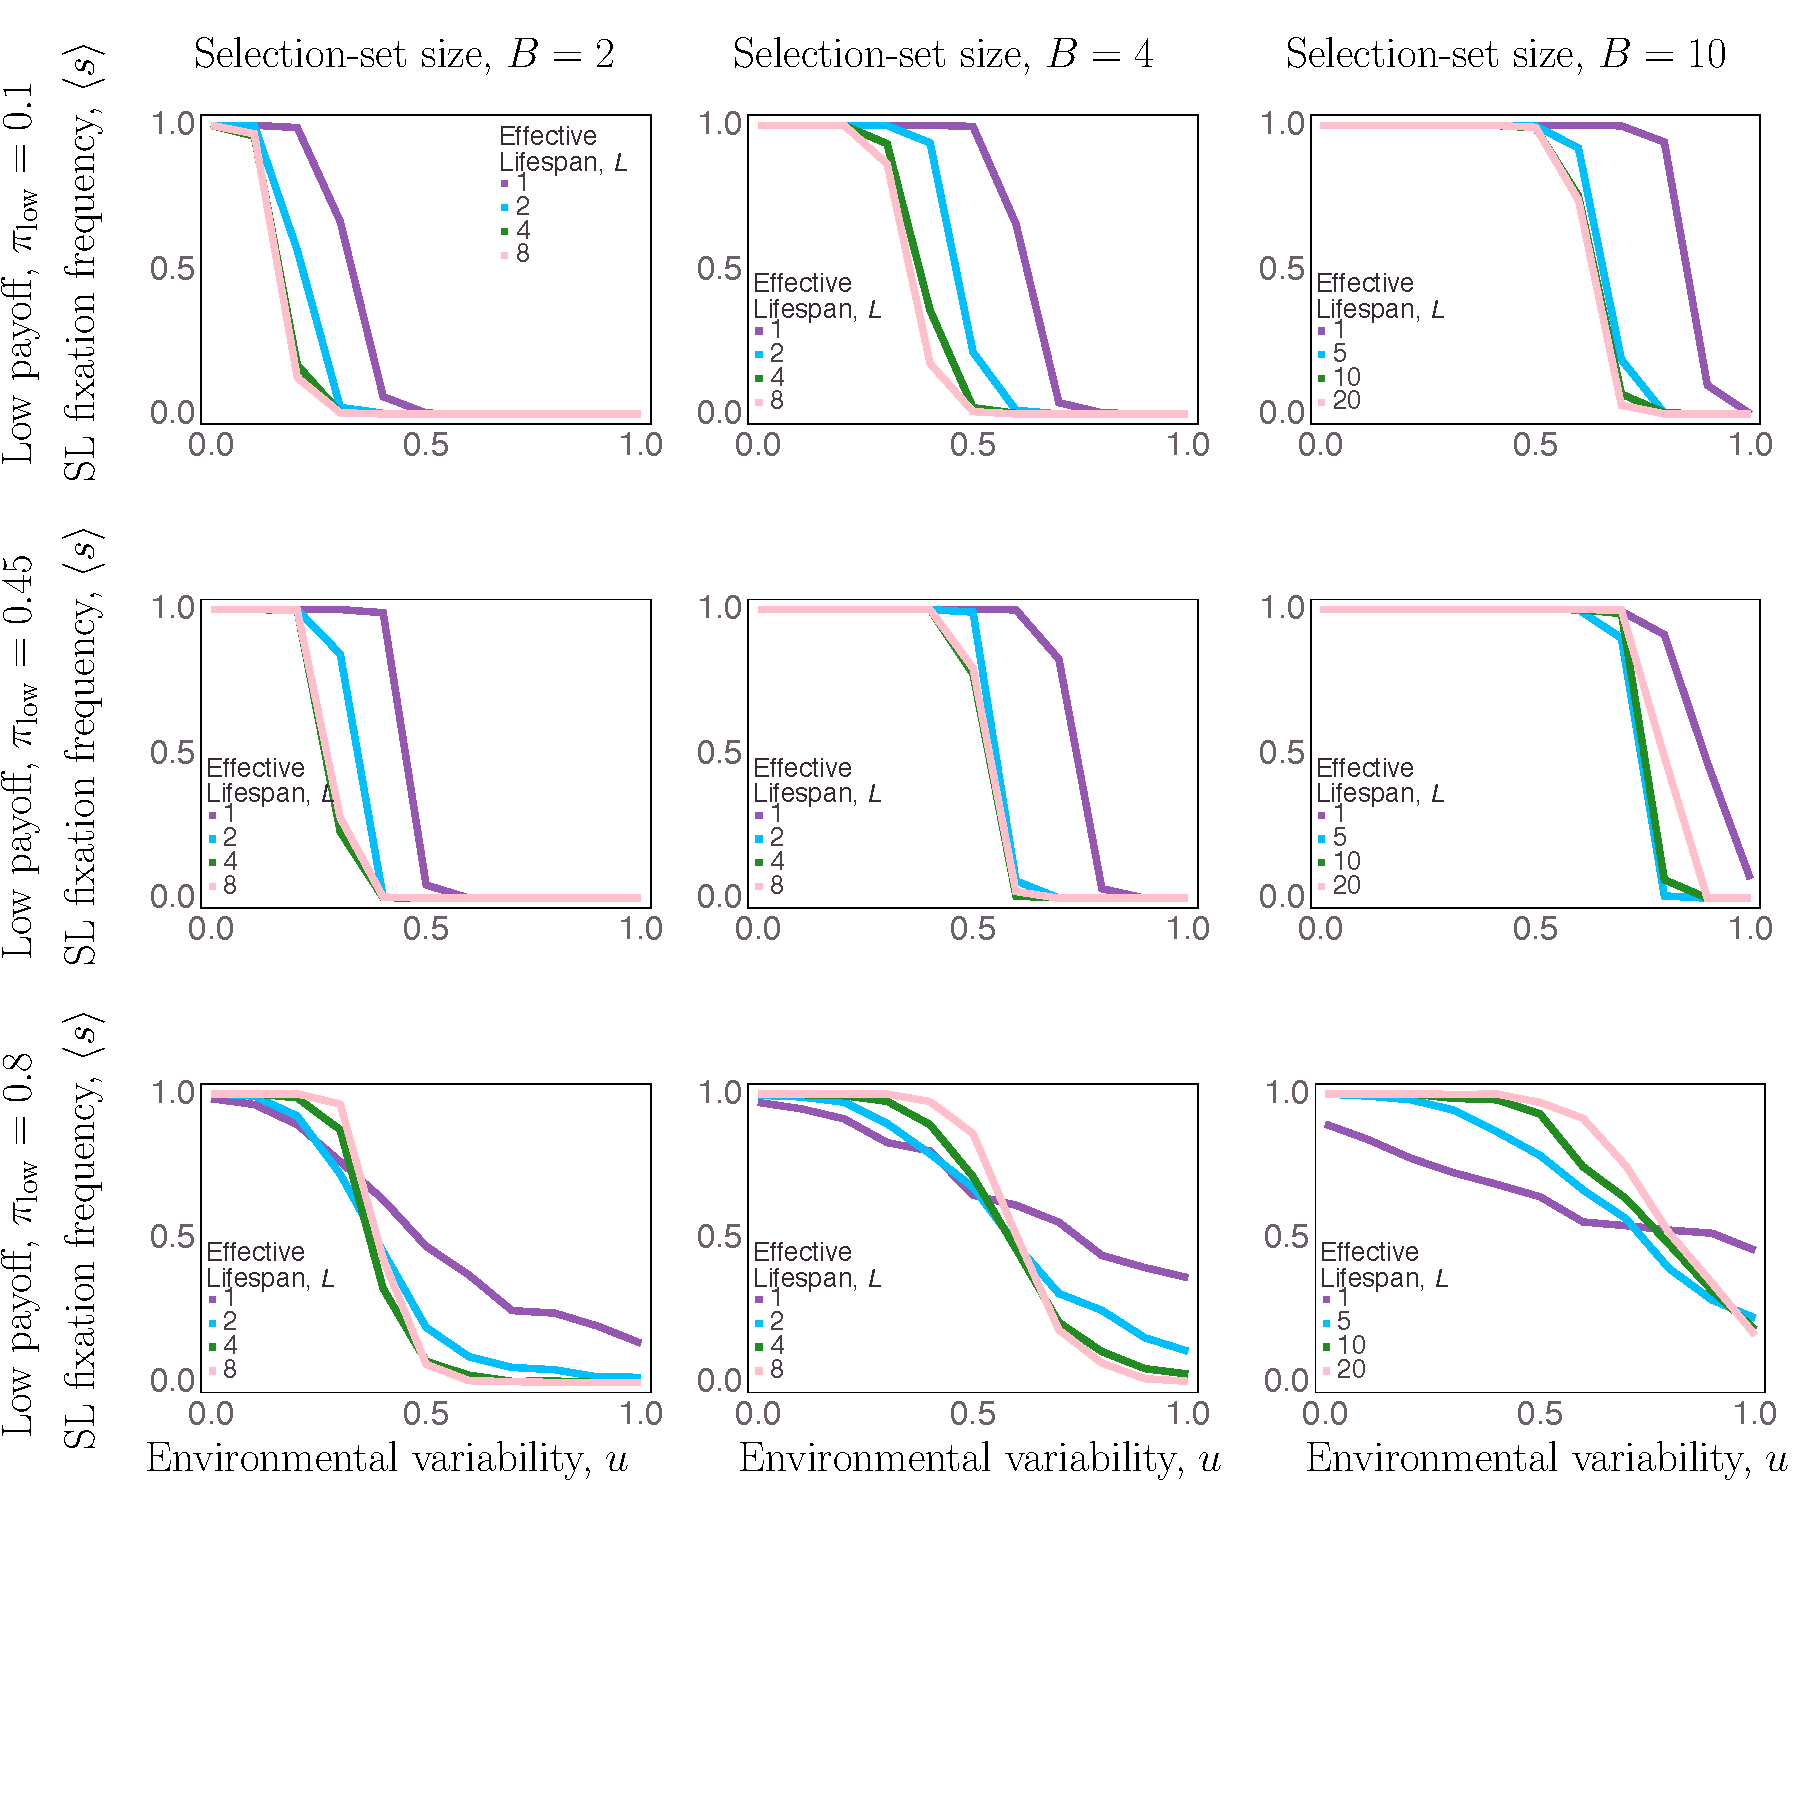
\includegraphics[width=\textwidth]{Figures/supplement/nteachers=2/mainResultsPlots.pdf}
  \end{subfigure}
\end{figure}
% \newpage
% \begin{figure}
%   \ContinuedFloat
%   \begin{subfigure}{\textwidth}
% 	\caption{$N_T = 10$}
% 	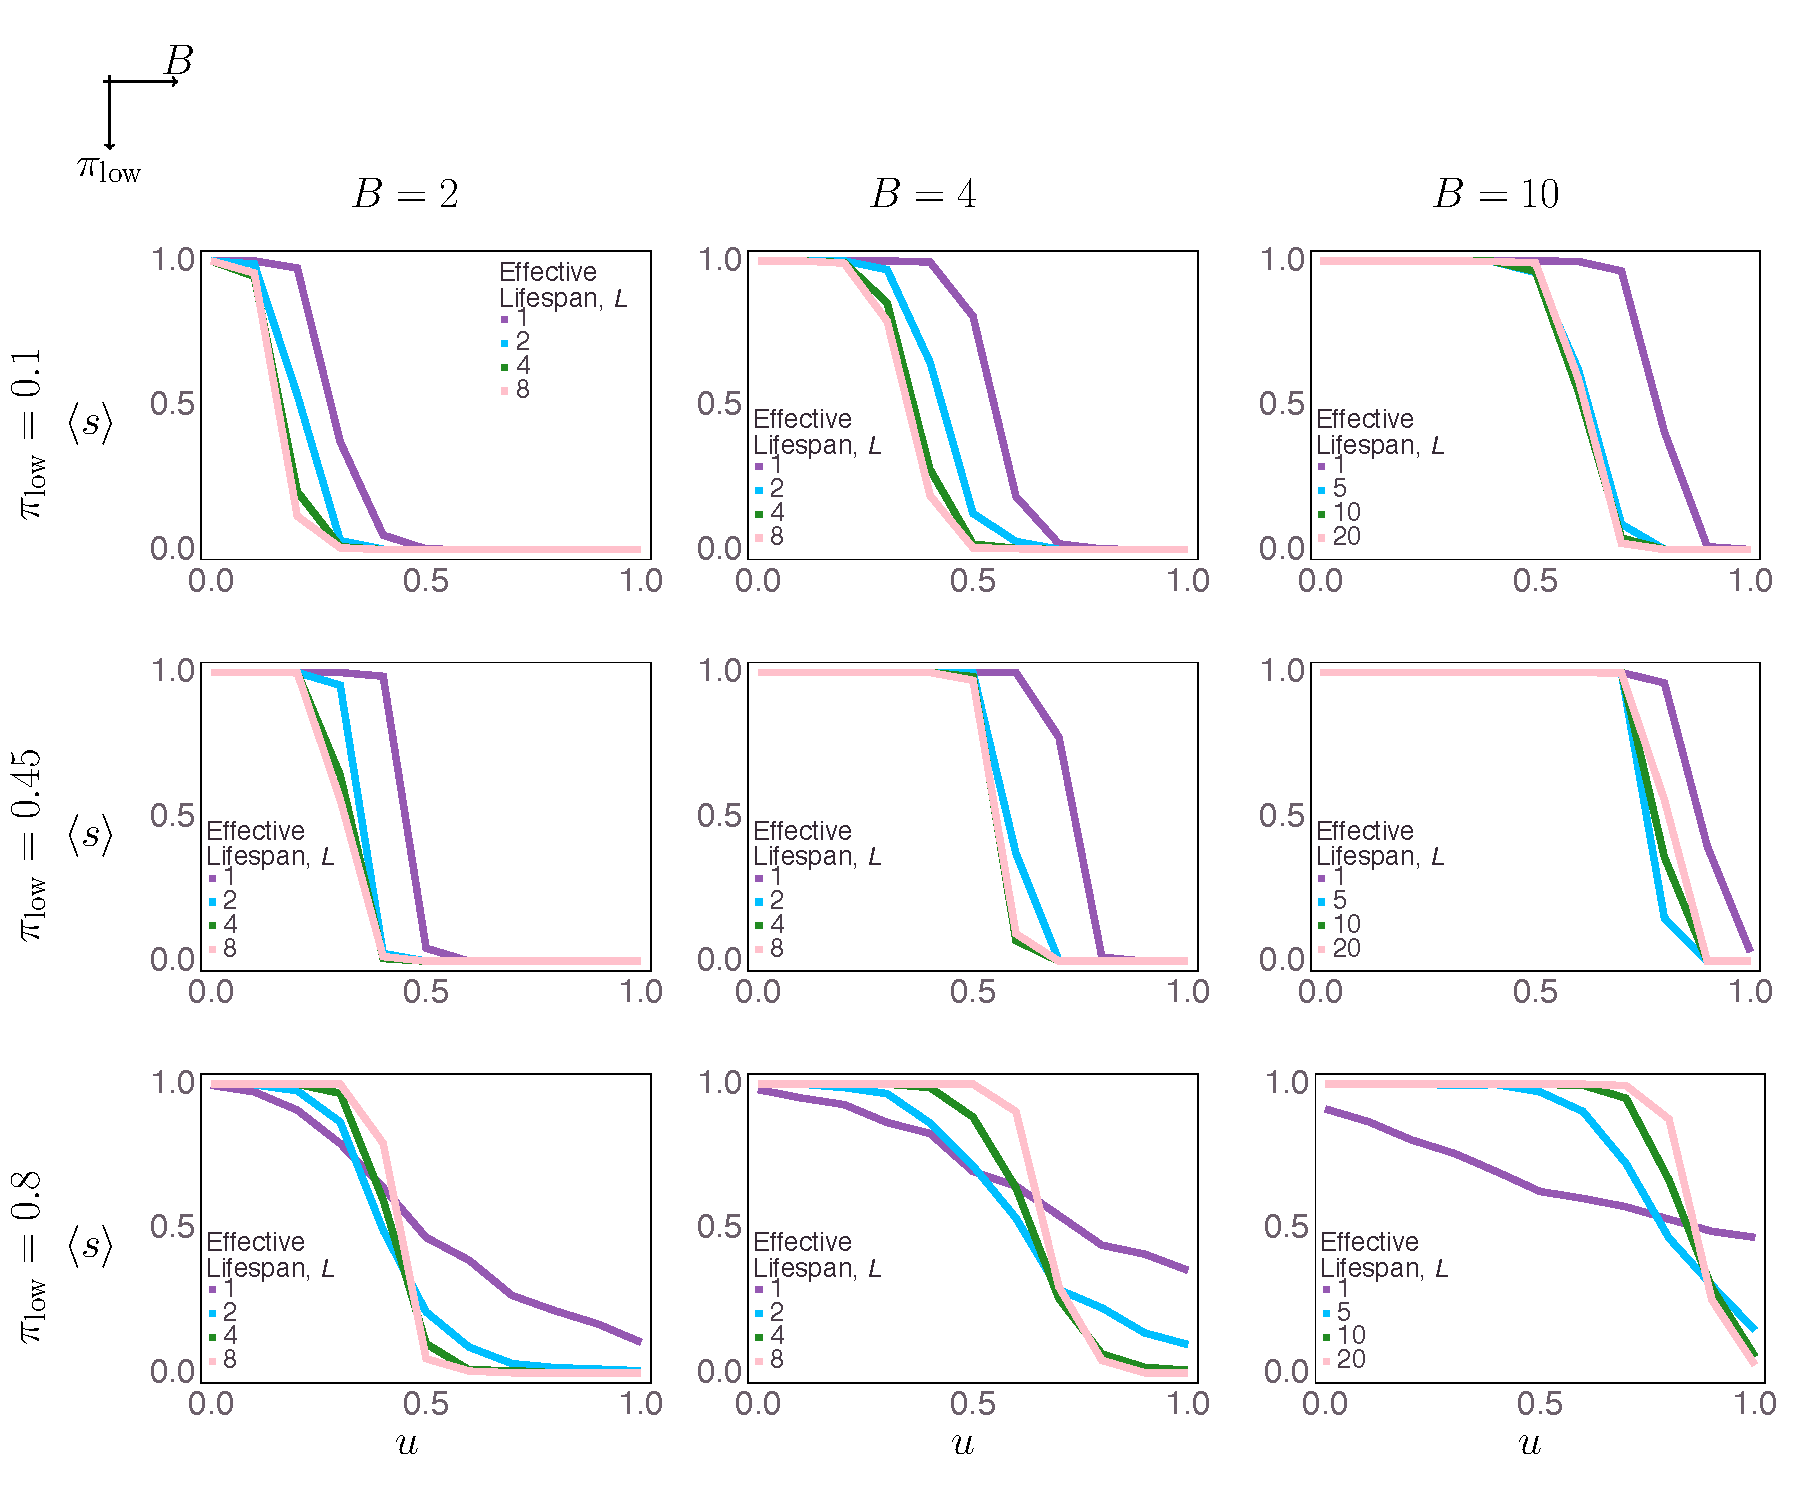
\includegraphics[width=\textwidth]{Figures/supplement/nteachers=10/mainResultsPlots.pdf}
%   \end{subfigure}
% \end{figure}
\newpage
\begin{figure}
  \ContinuedFloat
  \begin{subfigure}{\textwidth}
	\caption{$N_T = 20$}
	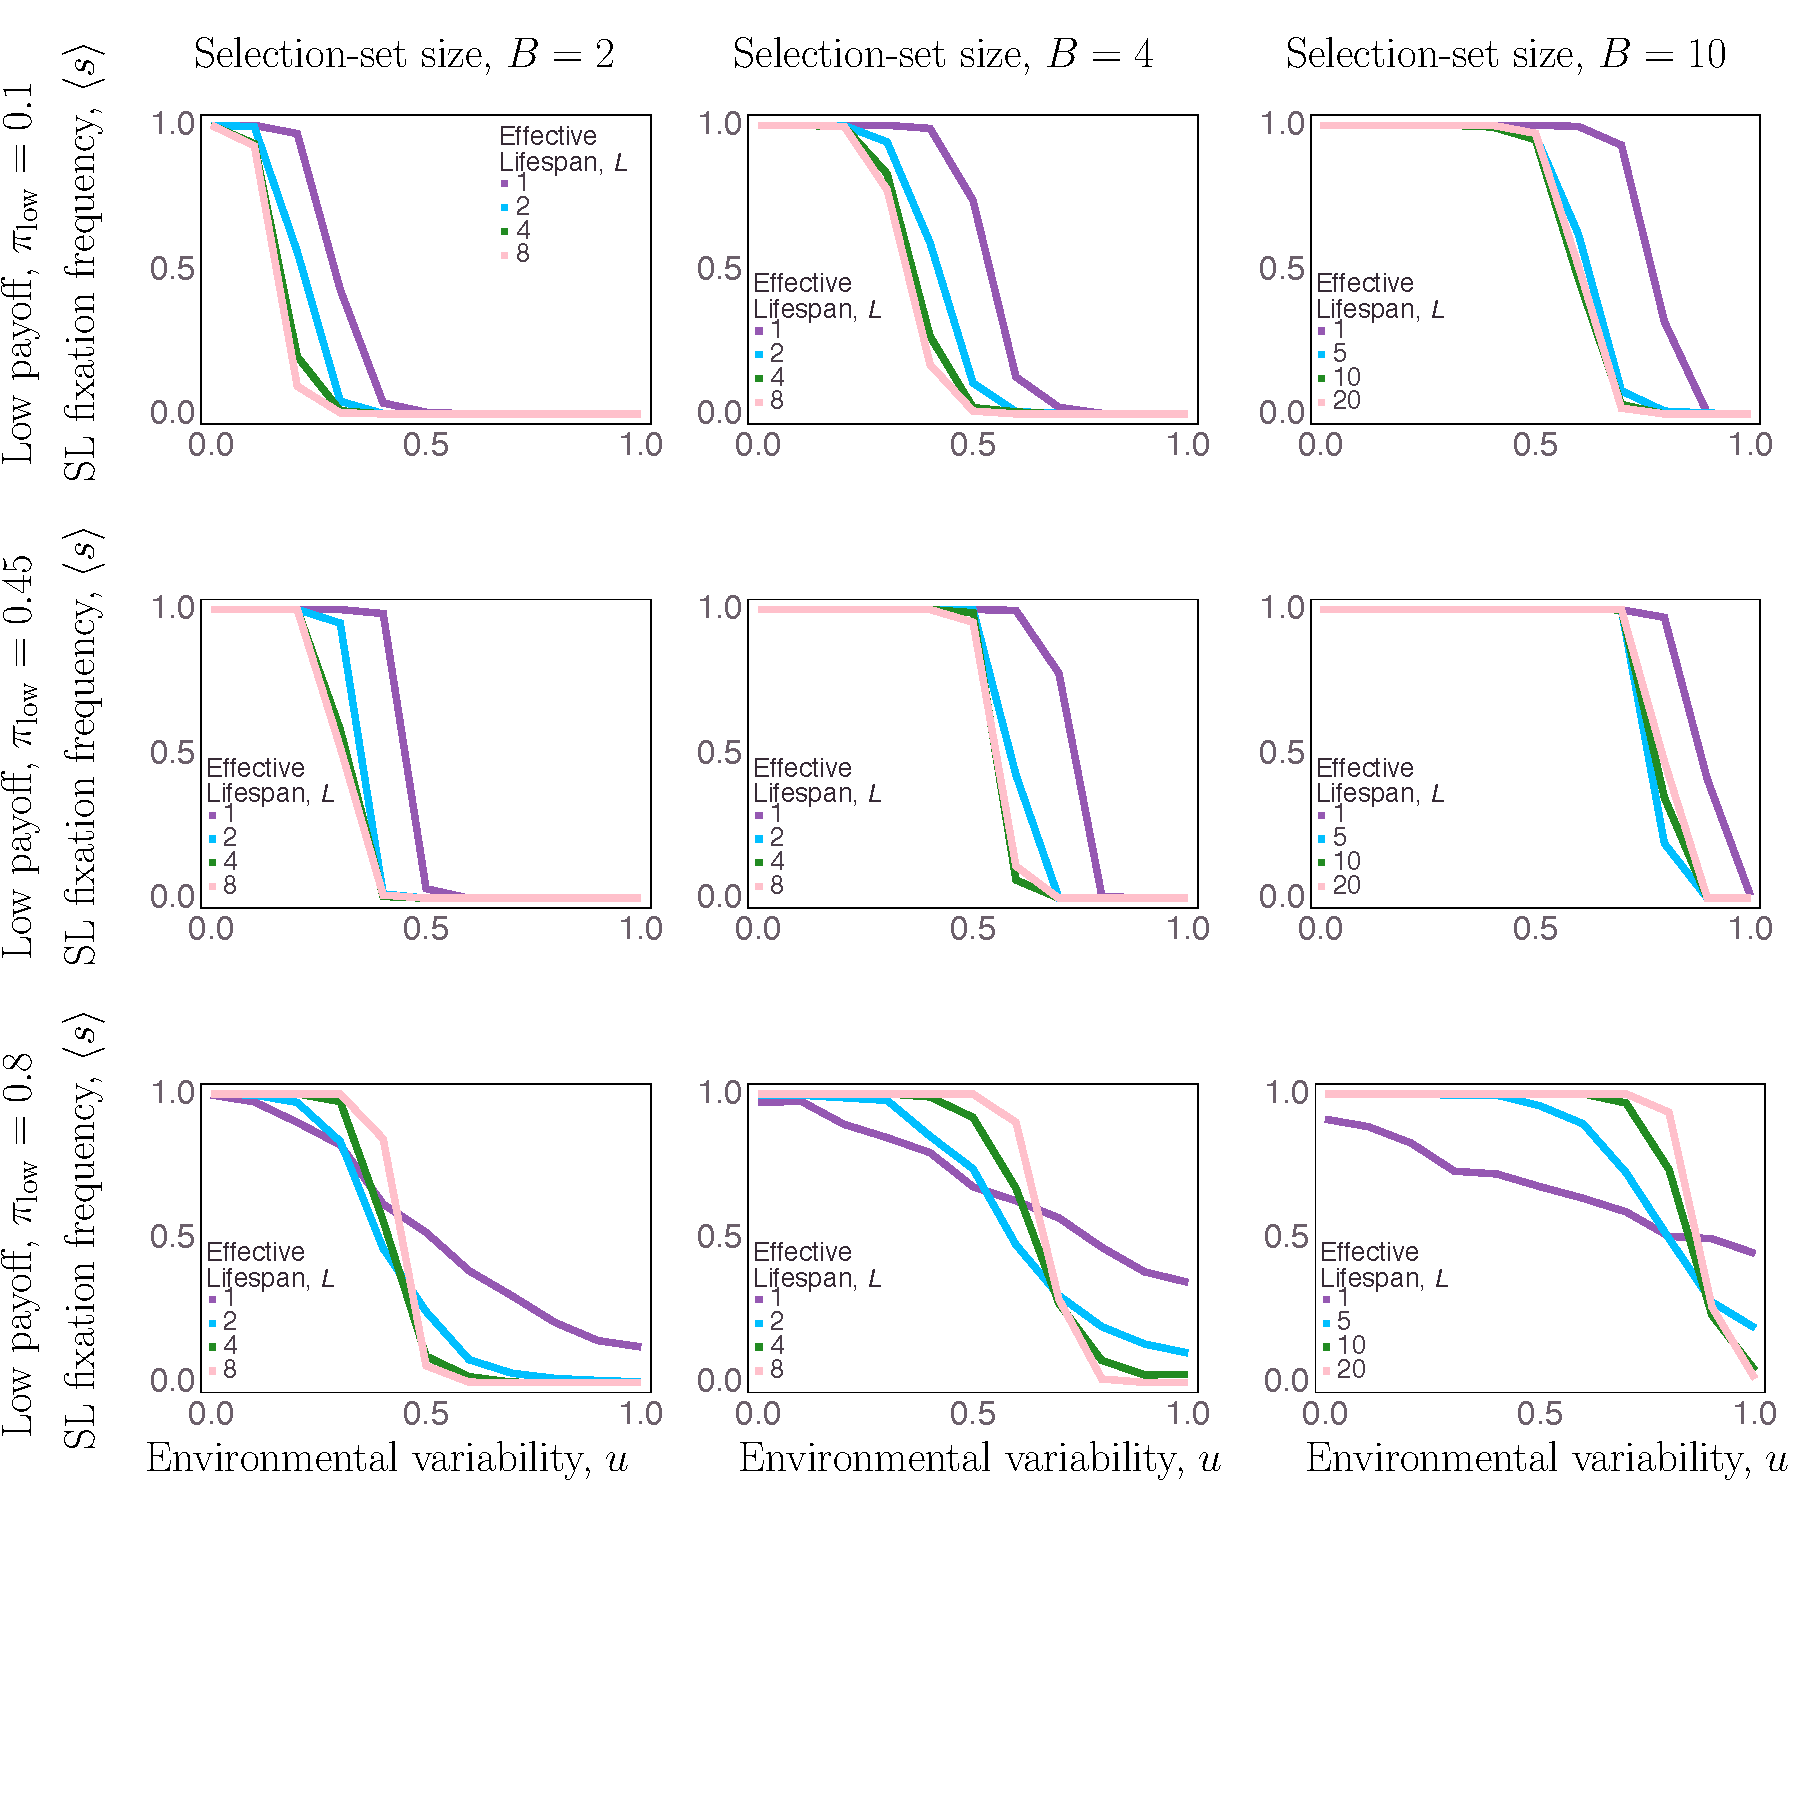
\includegraphics[width=\textwidth]{Figures/supplement/nteachers=20/mainResultsPlots.pdf}
  \end{subfigure}
\end{figure}

\clearpage


\section{Softmax parameter sensitivity analysis} 

We tested two additional settings of the softmax behavior selection greediness parameter,
$\beta=1,100$, which reproduced qualitative patterns in the evolution of social learning
observed in the main text where we used $\beta=10$.  
Softmax greediness is achieved formally by increasing the
probability mass for selecting behaviors that have paid off more frequently over that agent's
life history. In other words, greater $\beta$ increases the probabilty that the optimal
observed behavior is chosen over all the rest. If $\beta$ is too small, agents will fail to
fully exploit their knowledge about which behavior is optimal because they too frequently
explore less profitable alternatives.  If $\beta$ is too great the agents may prematurely
settle on a sub-optimal behavior because it paid off first.  In a fuller evolutionary
exploration of model parameters one might allow $\beta$ to co-evolve, through
mutation and selection, with the social learner trait.  
However, our sensitivity analysis suggests this would be unnecessary 
since our main conclusions of how social learning evolves under uncertainty remain unchanged for different
$\beta$ over three orders of magnitude.

First, when $\beta=1$, most general trends are preserved, but in many cases the evolution
of social learning is suppressed or drift dominates due to 
due to the overall poor quality of information acquired through softmax search-based
individual learning. This increased drift is especially pronounced 
when $\pilow=0.8$ since sub-optimal behaviors often pay off and $\beta=1$ is
not aggressive enough to efficiently detect and exploit the optimal 
behavior (Figure~\ref{fig:softmaxSensitivity}a, bottom row).
Similarly, when $\beta = 1$, social learning is suppressed at much smaller values
of $u$ for longer lifespans, $L$, due to maximal excessive exploration of non-optimal
behaviors under this setting (Figure~\ref{fig:softmaxSensitivity}a, columns 
for $B$ and inset for $L$).

The main results were again qualitatively obtained again with $\beta=100$
(Figure~\ref{fig:softmaxSensitivity}b). 
In some cases, especially when $\pilow=0.1$, individual learning may be performing
better with $\beta=100$ compared to results in the main text ($\beta=10$), 
evidenced by a quicker decline of social learning prevalence over $u$ when
$L > 1$ (Figure~\ref{fig:softmaxSensitivity}b,
top row).
 


\vspace{-3em} \begin{figure} %\addtocounter{figure}{-1} 
  \centering
  \caption{Sensitivity analysis of the main results for the softmax parameter $\beta = 100$ and
  % \addtocounter{figure}{-1}
  $\beta=1$. Recall the main results were obtained with $\beta = 10$.}
  \label{fig:softmaxSensitivity} \vspace{2em}
  \begin{subfigure}{\textwidth}
	\caption{$\beta = 1$}
	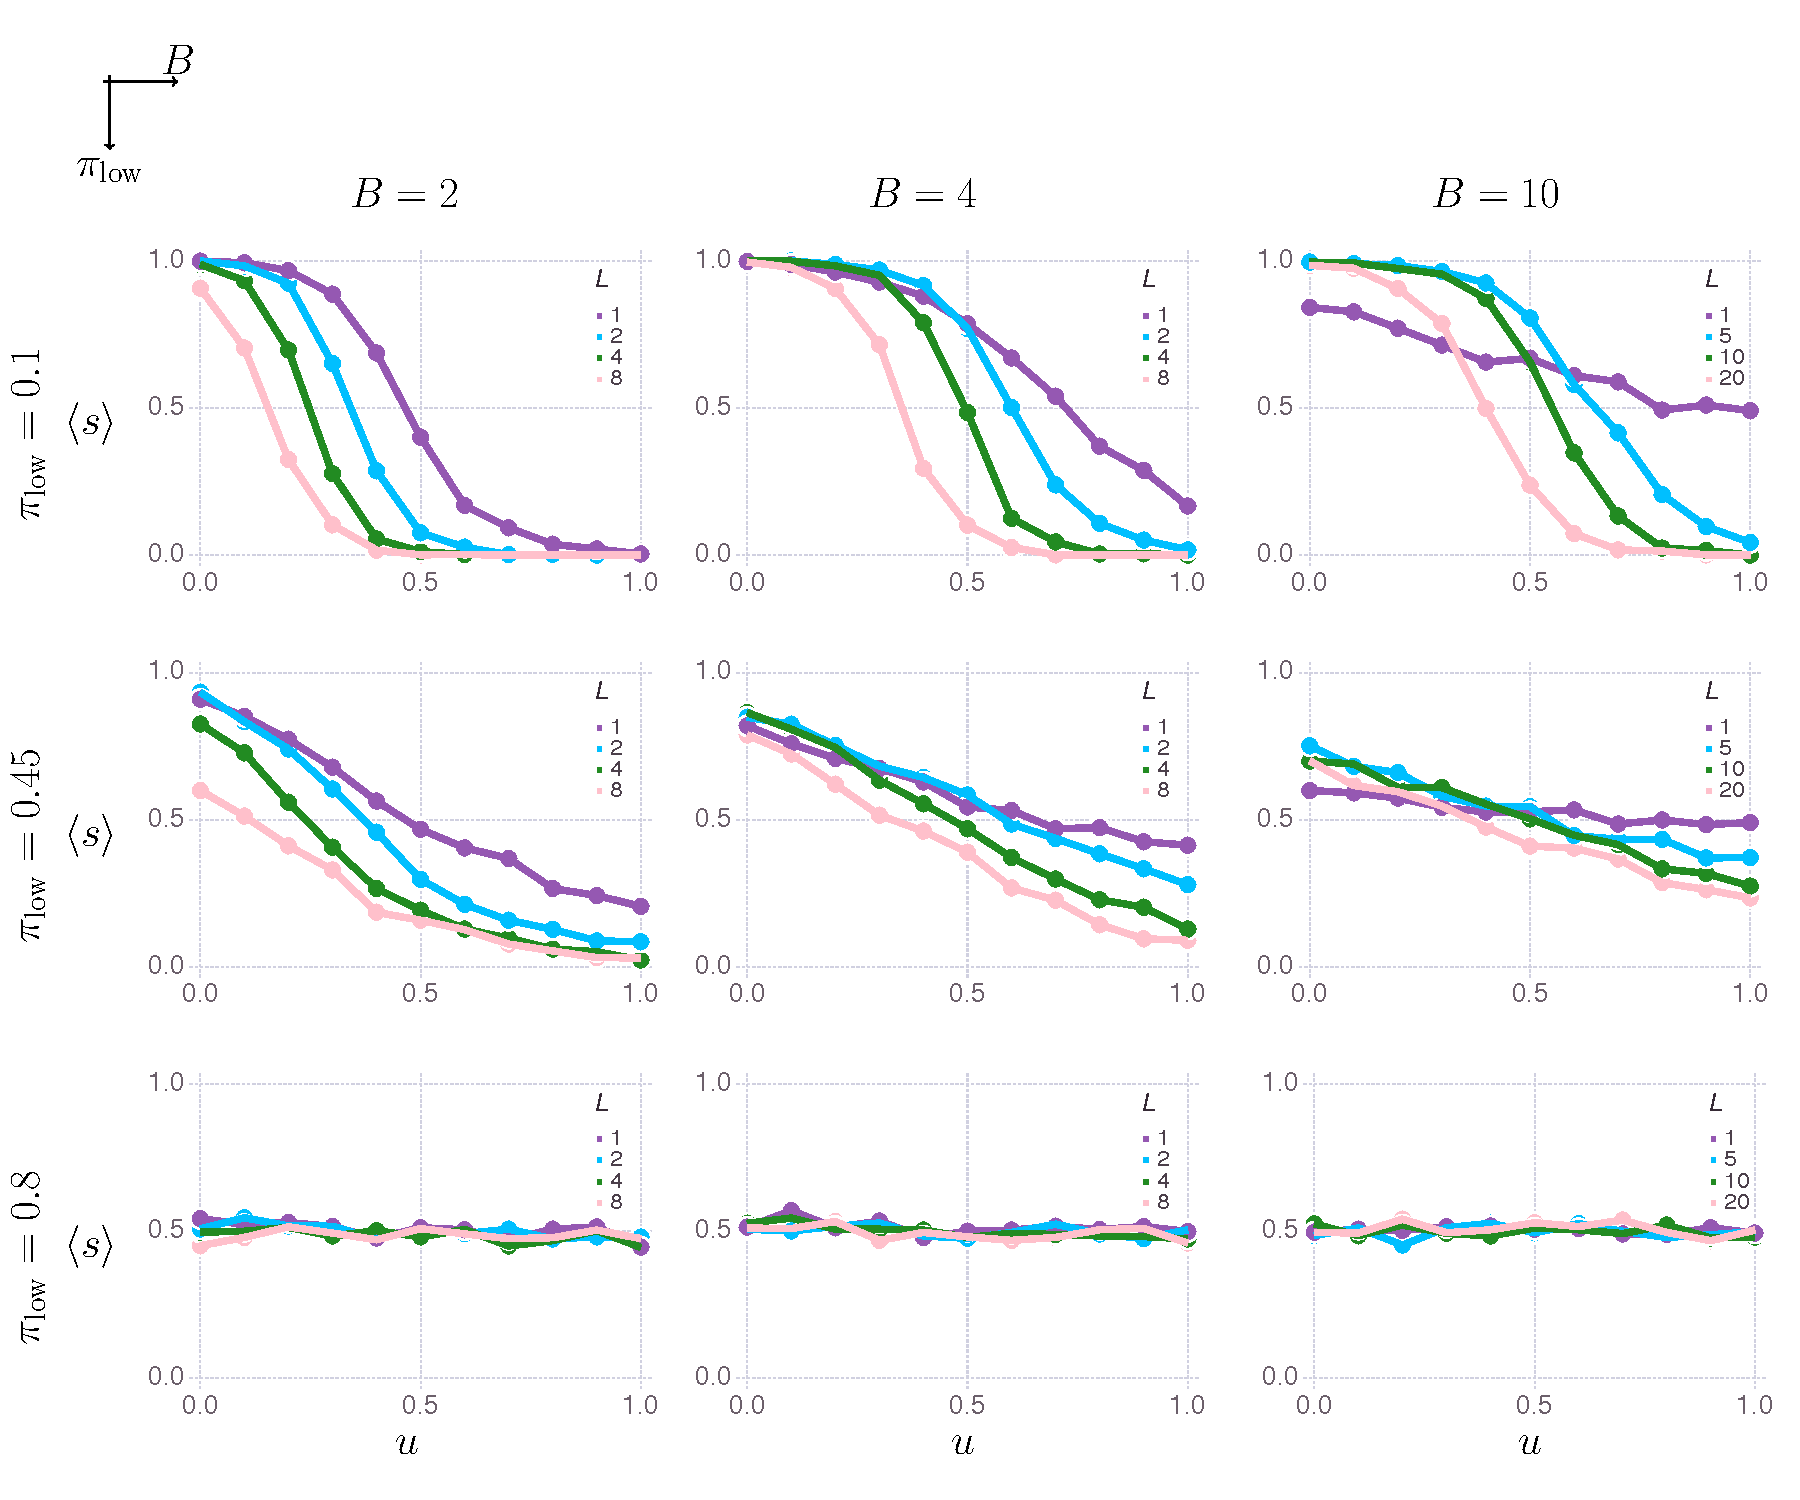
\includegraphics[width=\textwidth]{Figures/supplement/sensitivity_tau=1.0/mainResultsPlots.pdf}
  \end{subfigure}
\end{figure}
\newpage
\begin{figure}
  \ContinuedFloat
  \begin{subfigure}{\textwidth}
	\caption{$\beta = 100$}
	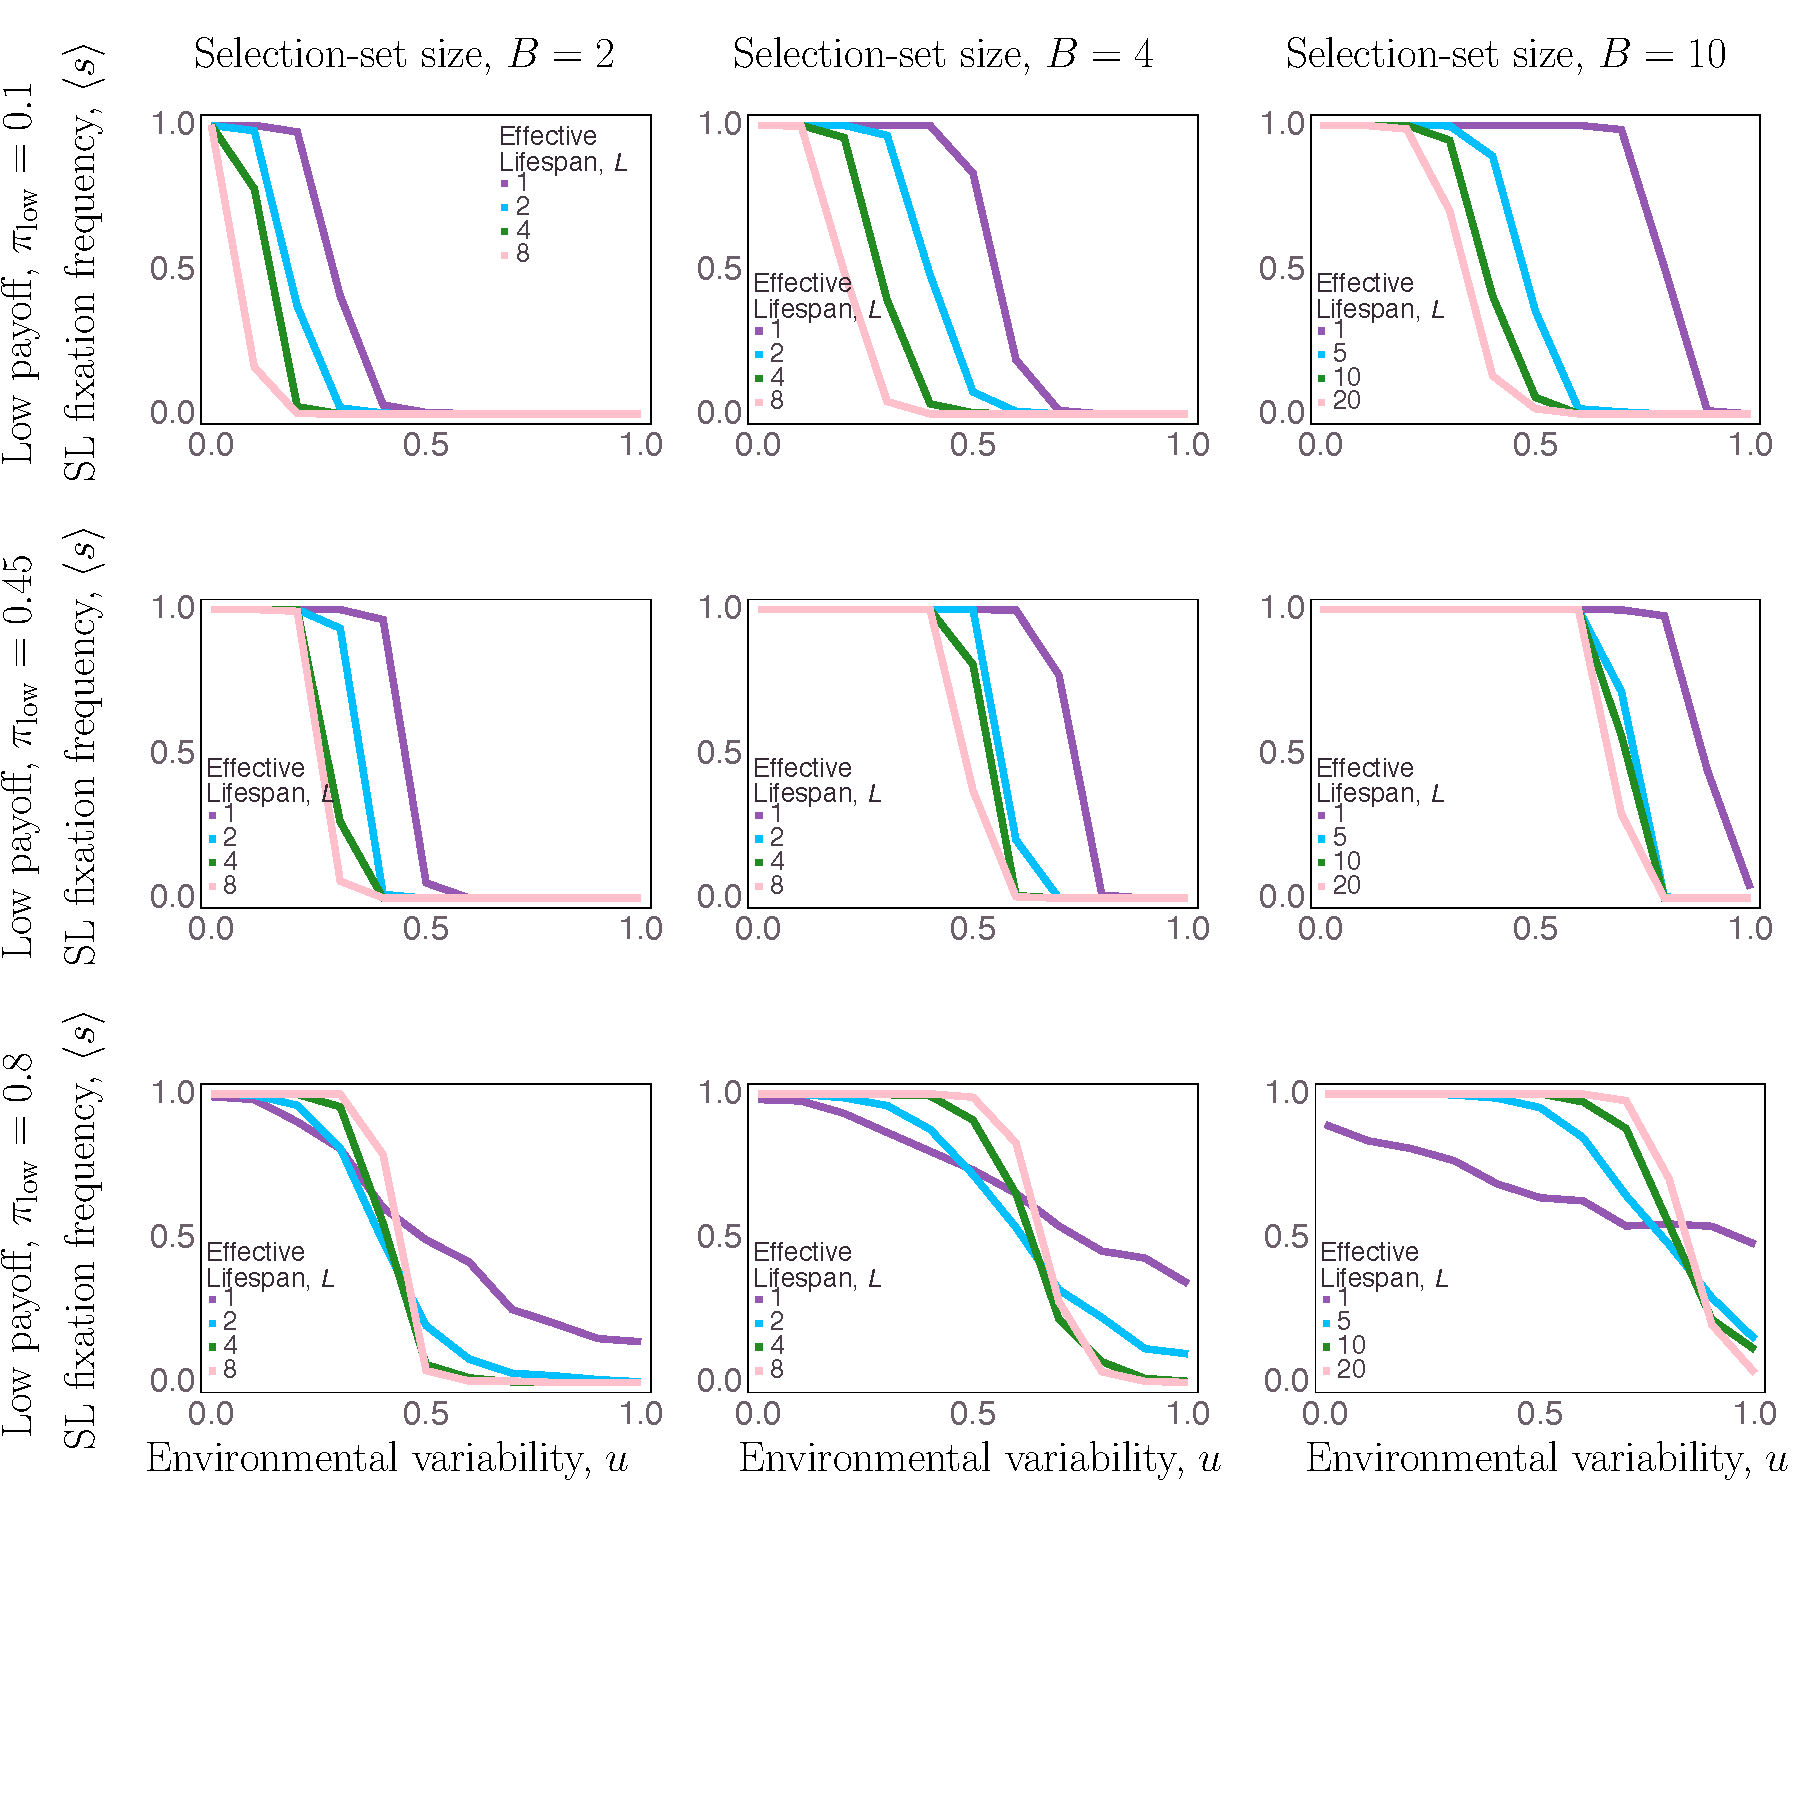
\includegraphics[width=\textwidth]{Figures/supplement/sensitivity_tau=0.01/mainResultsPlots.pdf}
  \end{subfigure}
\end{figure}



\end{document}
